% Aberdeen style guide should be followed when using this
% layout. Their template powerpoint slide is used to extract the
% Aberdeen color and logo but is otherwise ignored (it has little or
% no formatting in it anyway).
%
% http://www.abdn.ac.uk/documents/style-guide.pdf

%%%%%%%%%%%%%%%%%%%% Document Class Settings %%%%%%%%%%%%%%%%%%%%%%%%%
% Pick if you want slides, or draft slides (no animations)
%%%%%%%%%%%%%%%%%%%%%%%%%%%%%%%%%%%%%%%%%%%%%%%%%%%%%%%%%%%%%%%%%%%%%%
%Normal document mode
\documentclass[10pt,compress]{beamer}
%\documentclass[10pt,compress,handout]{beamer}
%%%%%Draft or handout mode
%\documentclass[10pt,compress,handout,ignorenonframetext]{beamer}

%%%%%%%%%%%%%%%%%%%% General Document settings %%%%%%%%%%%%%%%%%%%%%%%
% These settings must be set for each presentation
%%%%%%%%%%%%%%%%%%%%%%%%%%%%%%%%%%%%%%%%%%%%%%%%%%%%%%%%%%%%%%%%%%%%%%

\newcommand{\shortname}{Dr Jeff Gomes}
\newcommand{\fullname}{Dr Jeff Gomes}
\institute{School of Engineering}
\newcommand{\emailaddress}{jefferson.gomes@abdn.ac.uk}
\newcommand{\logoimage}{../FigBanner/UoAHorizBanner}
\title{Engineering Thermodynamics (EG3521)}
\subtitle{Module 2: Production of Power from Heat}
\date[24-28/02/2014]{24-28 February 2014}

%%%%%%%%%%%%%%%%%%%% Template settings %%%%%%%%%%%%%%%%%%%%%%%%%%%%%%%
% You shouldn't have to change below this line, unless you want to.
%%%%%%%%%%%%%%%%%%%%%%%%%%%%%%%%%%%%%%%%%%%%%%%%%%%%%%%%%%%%%%%%%%%%%%
\usecolortheme{whale}
\useoutertheme{infolines}

% Use the fading effect for items that are covered on the current
% slide.
\beamertemplatetransparentcovered

% We abuse the author command to place all of the slide information on
% the title page.
\author[\shortname]{%
  \fullname\\\ttfamily{\emailaddress}
}


%At the start of every section, put a slide indicating the contents of the current section.
%\AtBeginSection[] {
%  \begin{frame}
%    \frametitle{Section Outline}
%    \tableofcontents[currentsection]
%  \end{frame}
%}

% Allow the inclusion of movies into the Presentation! At present,
% only the Okular program is capable of playing the movies *IN* the
% presentation.
\usepackage{multimedia}
\usepackage{animate}

% \usepackage[usenames,dvipsnames]{pstricks}
% \usepackage{epsfig}
% \usepackage{pst-grad} % For gradients
% \usepackage{pst-plot} % For axes


%%%%% Color settings
\usepackage{color}
%% The background color for code listings (i.e. example programs)
\definecolor{lbcolor}{rgb}{0.9,0.9,0.9}%
\definecolor{UoARed}{rgb}{0.64706, 0.0, 0.12941}
\definecolor{UoALight}{rgb}{0.85, 0.85, 0.85}
\definecolor{UoALighter}{rgb}{0.92, 0.92, 0.92}
\setbeamercolor{structure}{fg=UoARed} % General background and higlight color
\setbeamercolor{frametitle}{bg=black} % General color
\setbeamercolor{frametitle right}{bg=black} % General color
\setbeamercolor{block body}{bg=UoALighter} % For blocks
\setbeamercolor{structure}{bg=UoALight} % For blocks
% Rounded boxes for blocks
\setbeamertemplate{blocks}[rounded]

%%%%% Font settings
\newcommand{\frc}{\displaystyle\frac}
% Aberdeen requires the use of Arial in slides. We can use the
% Helvetica font as its widely available like so
% \usepackage{helvet}
% \renewcommand{\familydefault}{\sfdefault}
% But beamer already uses a sans font, so we will stick with that.

% The size of the font used for the code listings.
\newcommand{\goodsize}{\fontsize{6}{7}\selectfont}

% Extra math packages, symbols and colors. If you're using Latex you
% must be using it for formatting the math!
\usepackage{amscd,amssymb} \usepackage{amsfonts}
\usepackage[mathscr]{eucal} \usepackage{mathrsfs}
\usepackage{latexsym} \usepackage{amsmath} \usepackage{bm}
\usepackage{amsthm} \usepackage{textcomp} \usepackage{eurosym}
% This package provides \cancel{a} and \cancelto{a}{b} to "cancel"
% expressions in math.
\usepackage{cancel}

% Get rid of font warnings as modern LaTaX installations have scalable
% fonts
\usepackage{type1cm} 

%\usepackage{enumitem} % continuous numbering throughout enumerate commands

% For exact placement of images/text on the cover page
\usepackage[absolute]{textpos}
\setlength{\TPHorizModule}{1mm}%sets the textpos unit
\setlength{\TPVertModule}{\TPHorizModule} 

% Source code formatting package
\usepackage{listings}%
\lstset{ backgroundcolor=\color{lbcolor}, tabsize=4,
  numberstyle=\tiny, rulecolor=, language=C++, basicstyle=\goodsize,
  upquote=true, aboveskip={1.5\baselineskip}, columns=fixed,
  showstringspaces=false, extendedchars=true, breaklines=false,
  prebreak = \raisebox{0ex}[0ex][0ex]{\ensuremath{\hookleftarrow}},
  frame=single, showtabs=false, showspaces=false,
  showstringspaces=false, identifierstyle=\ttfamily,
  keywordstyle=\color[rgb]{0,0,1},
  commentstyle=\color[rgb]{0.133,0.545,0.133},
  stringstyle=\color[rgb]{0.627,0.126,0.941}}

% Allows the inclusion of other PDF's into the final PDF. Great for
% attaching tutorial sheets etc.
\usepackage{pdfpages}
\setbeamercolor{background canvas}{bg=}  

% Remove foot note horizontal rules, they occupy too much space on the slide
\renewcommand{\footnoterule}{}

% Force the driver to fix the colors on PDF's which include mixed
% colorspaces and transparency.
\pdfpageattr {/Group << /S /Transparency /I true /CS /DeviceRGB>>}

% Include a graphics, reserve space for it but
% show it on the next frame.
% Parameters:
% #1 Which slide you want it on
% #2 Previous slides
% #3 Options to \includegraphics (optional)
% #4 Name of graphic
\newcommand{\reserveandshow}[4]{%
\phantom{\includegraphics<#2|handout:0>[#3]{#4}}%
\includegraphics<#1>[#3]{#4}%
}

\begin{document}

% Title page layout
\begin{frame}
  \titlepage
  \vfill%
  \begin{center}
    \includegraphics[clip,width=0.8\textwidth]{\logoimage}
  \end{center}
\end{frame}

% Table of contents
%\frame{ \frametitle{Slides Outline}
%  \tableofcontents
%}


%%%%%%%%%%%%%%%%%%%% The Presentation Proper %%%%%%%%%%%%%%%%%%%%%%%%%
% Fill below this line with \begin{frame} commands! It's best to
% always add the fragile option incase you're going to use the
% verbatim environment.
%%%%%%%%%%%%%%%%%%%%%%%%%%%%%%%%%%%%%%%%%%%%%%%%%%%%%%%%%%%%%%%%%%%%%%

\section{Module 2.2.2: Gas-Turbine Power Systems}

%%%
%%% Slide
%%%
\subsection{Motivation}
\begin{frame}
 \frametitle{Aims and Objectives}
 At the end of this lecture, you should be able to:
 \begin{enumerate}[(i)]
  \item <1-> Understand how gas power cycles work;
  \item <2-> Solve problems based on the Brayton cycle;
  \item <3-> Identify simplifying assumptions for second-law analysis of gas power cycles.
  %\item <5-> 
 \end{enumerate}
\end{frame}

 
%%%
%%% Slide
%%%
\subsection{Bibliography} 
\begin{frame}
 \frametitle{Suggested References}
  Literature relevant for this module:
  \begin{enumerate}[(a)]
   \item J.M. Smith, H.C. Van Ness, M.M. Abbott, $\lq$Introduction to Chemical Engineering Thermodynamics', 6$^{th}$ Edition: Chapter 8;
   \item M.J. Moran, H.N. Saphiro, D.D. Boettner, M.B. Bailey, $\lq$Principles of Engineering Thermodynamics',  7$^{th}$ Edition: Chapter 9.
%
\item Y. Le Moullec (2013) \href{http://dx.doi.org/10.1016/j.energy.2012.10.022}{$\lq$Conceptual Study of a High Eficiency Coal-Fired Power Plant with CO$_{2}$ capture using Supercritical CO$_{2}$ Brayton Cycle'}, {\it Energy}, 49:32-46.
\item P. Spittle (2003) \href{http://dx.doi.org/10.1088/0031-9120/38/6/002}{$\lq$Gas Turbine Technology'}, {\it Physics Education}, 38:504-511.

  \end{enumerate}
\end{frame}



\subsection{Brayton Gas-Turbine Cycle}
%%%
%%% Slide
%%%
\begin{frame}
 \frametitle{Introduction}
 \begin{columns}
  \begin{column}[c]{0.6\linewidth} 
   \begin{itemize}
    \item <1-> Also called \textcolor{blue}{Joule cycle}, it is a constant pressure cycle initially designed for perfect gasses;
    \item <2-> Gas turbines usually operate on an open cycle: 
    \item <3-> Fresh air at ambient conditions is drawn into the compressor, where the temperature and pressure are raised;
    \item <4-> The \textcolor{blue}{high-pressure air} stream is injected into the combustion chamber, where the \textcolor{blue}{fuel is burned at constant pressure}; 
   \end{itemize}
  \end{column}
  \begin{column}[c]{0.4\linewidth}
   \begin{figure}%
    \vbox{
     \hbox{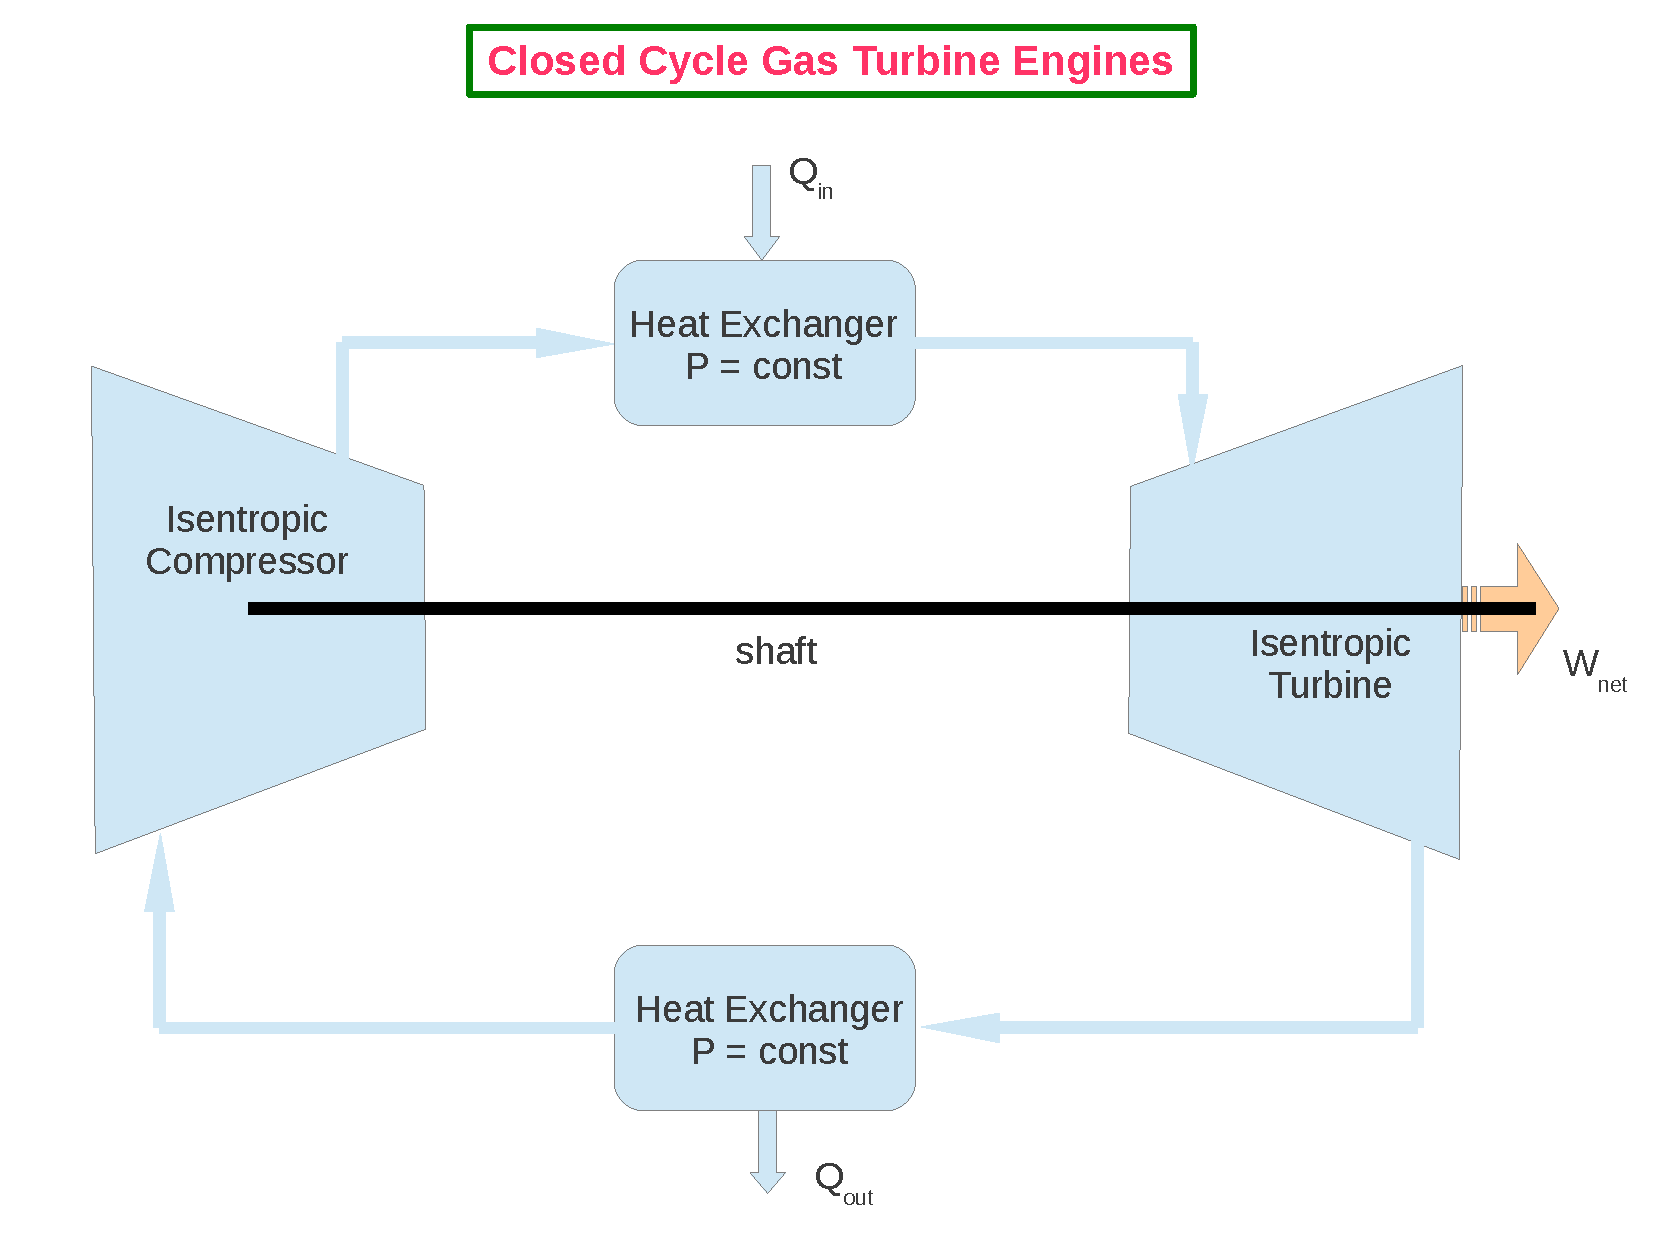
\includegraphics[width=5cm,clip]{./Pics/Closed_Gas_Turbine_Engines}}
     \hbox{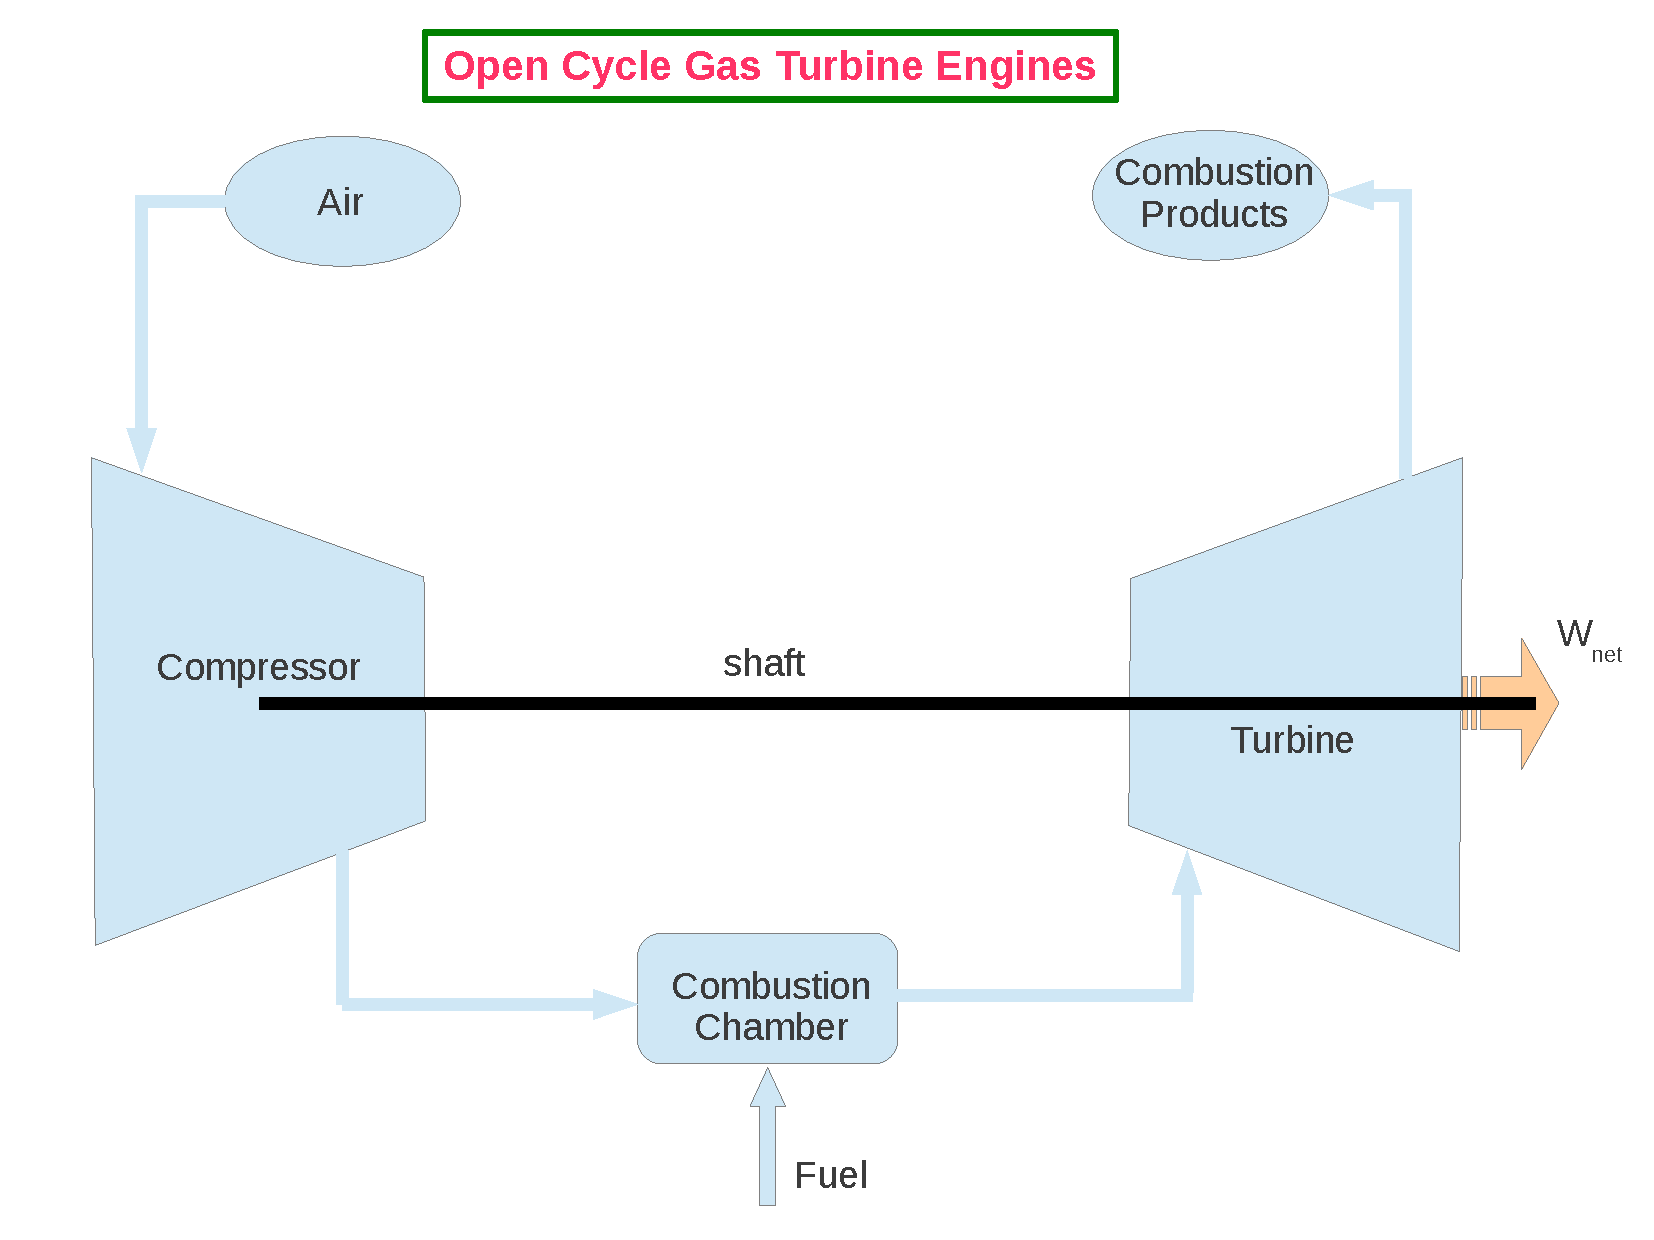
\includegraphics[width=5cm,clip]{./Pics/Open_Gas_Turbine_Engines}}
     }
   \end{figure}  
  \end{column}  
 \end{columns}
\end{frame}

%%%
%%% Slide
%%%
\begin{frame}
 \frametitle{Introduction}
 \begin{columns}
  \begin{column}[c]{0.6\linewidth} 
   \begin{itemize}
    \item <1-> The \textcolor{blue}{high-temperature combustion gasses} are directed into the \textcolor{blue}{turbine} where they \textcolor{blue}{isentropically expand to the atmospheric pressure};
    \item <2-> The exhaust gases leaving the turbine are discarded (not recirculated), therefore; 
    \item <3-> \textcolor{blue}{$\Longrightarrow$ Open Cycle $\Longleftarrow$}.
    \item <4-> However, we can simplify the open cycle by assuming air-standard assumptions where;
    \item <5-> \textcolor{blue}{The combustion stage is replaced by a constant-pressure heat-addition stage from an external source} and;
    \item <6-> \textcolor{blue}{The exhaust stage is replaced by a constant-pressure heat-rejection stage to the ambient air}.
   \end{itemize}
  \end{column}
  \begin{column}[c]{0.4\linewidth}
   \begin{figure}%
    \vbox{
     \hbox{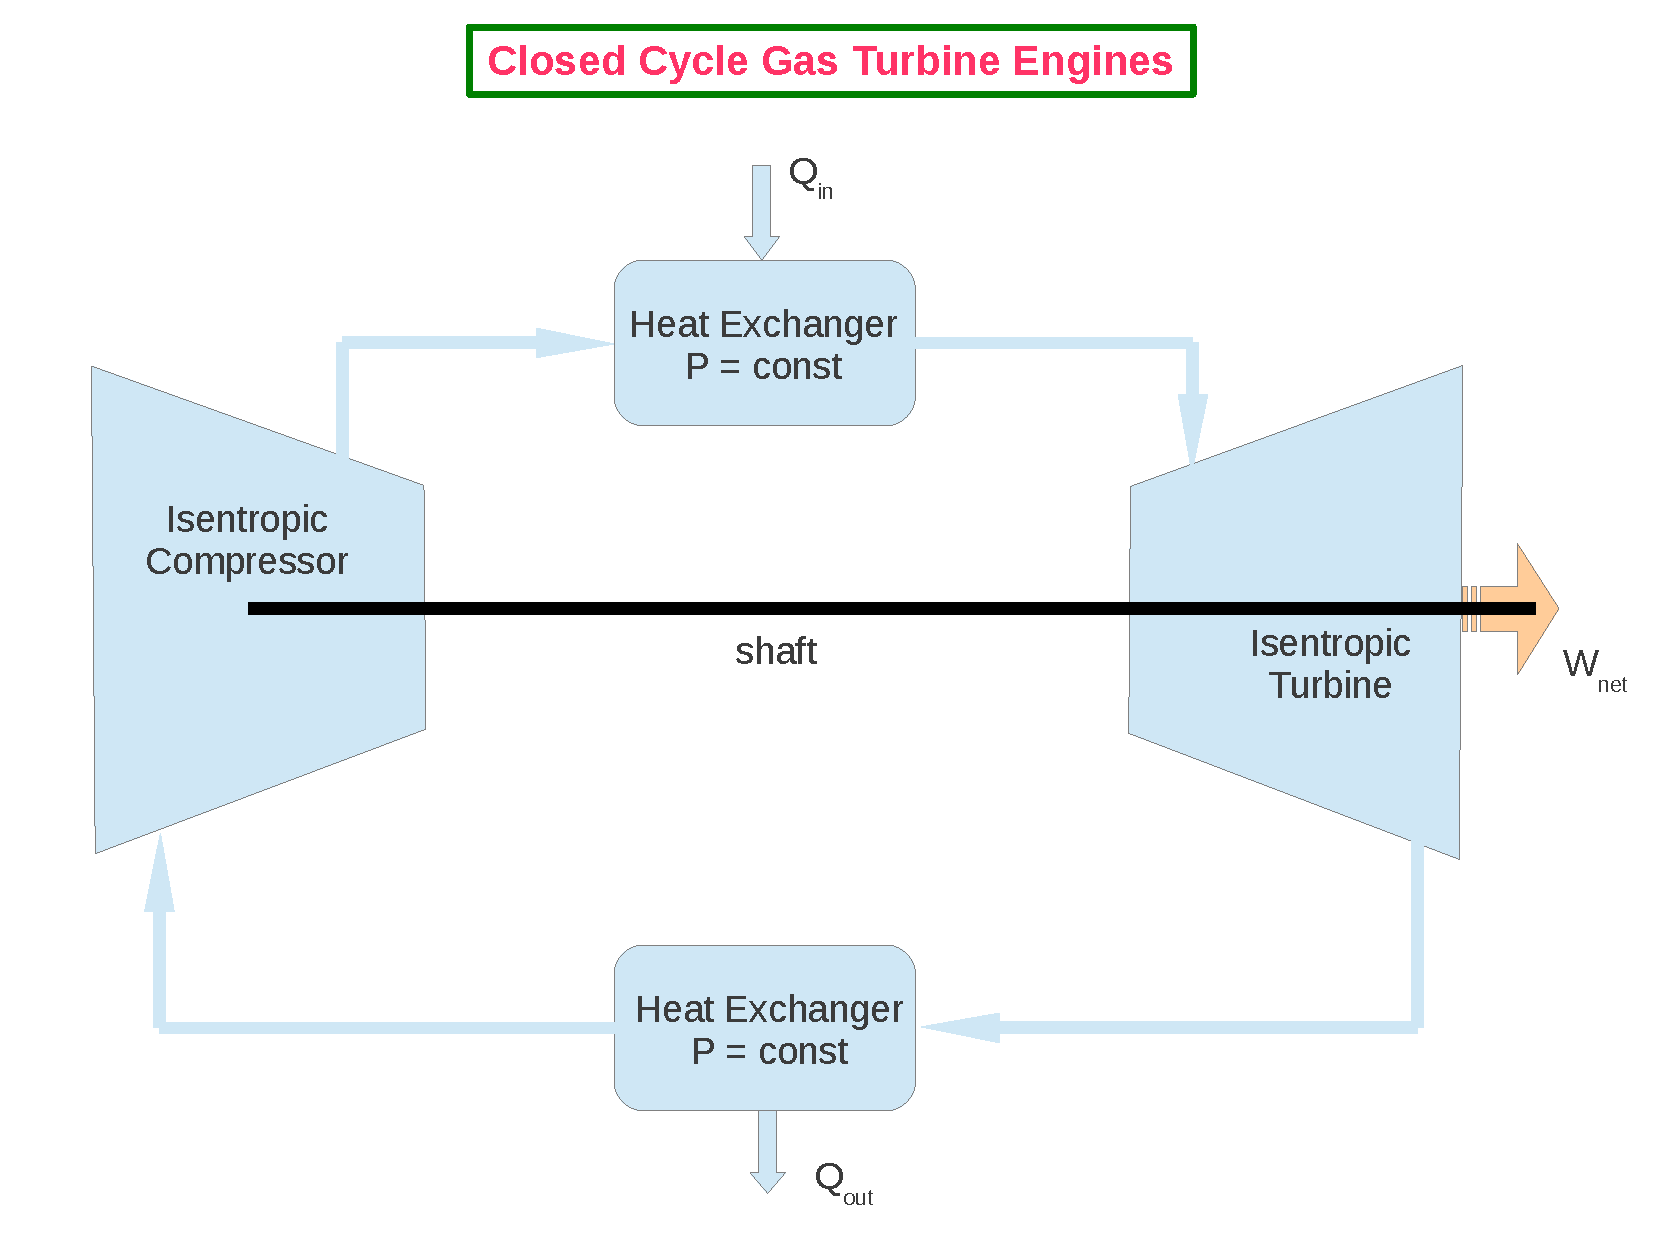
\includegraphics[width=5cm,clip]{./Pics/Closed_Gas_Turbine_Engines}}
     \hbox{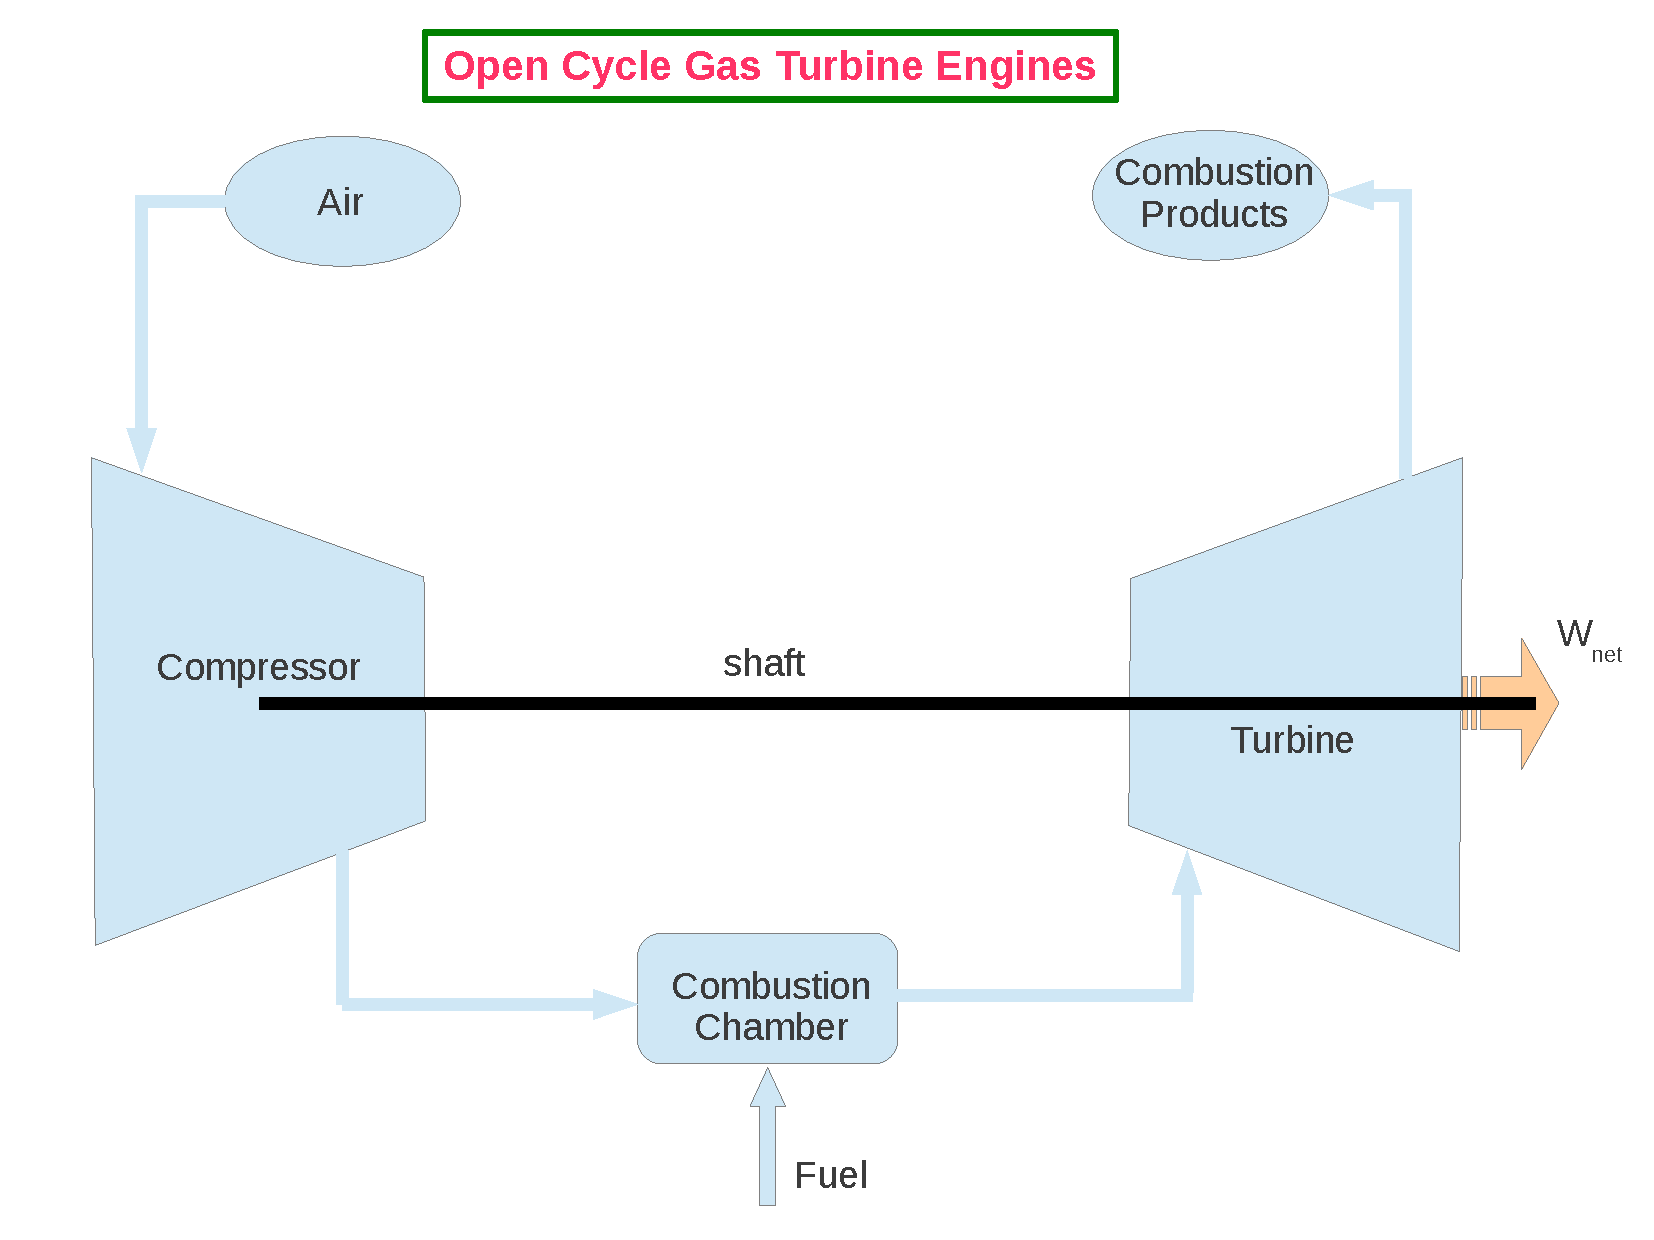
\includegraphics[width=5cm,clip]{./Pics/Open_Gas_Turbine_Engines}}
     }
   \end{figure}  
  \end{column}  
 \end{columns}
\end{frame}



%%%
%%% Slide
%%%
\begin{frame}
 \frametitle{Brayton Cycle -- Internally Reversible Processes}
 \begin{columns}
  \begin{column}[c]{0.4\linewidth} 
   \begin{itemize}
    \item <1-> \textcolor{blue}{1--2} Isentropic compression (compressor) of air from $\left(T_{1},P_{1},V_{1}\right)$ to $\left(T_{2},P_{2},V_{2}\right)$. No heat flow;
    \item <2-> \textcolor{blue}{2--3} Constant-pressure heat addition: heat flows into the system increasing the volume -- from $\left(T_{2},P_{2},V_{2}\right)$ to $\left(T_{3},P_{2}=P_{3},V_{3}\right)$.  \\
\textcolor{blue}{Heat received:} $Q_{in}=mC_{p}\left(T_{3}-T_{2}\right)$
   \end{itemize}
  \end{column}
  \begin{column}[c]{0.6\linewidth}
    \begin{center}
   \begin{figure}%
     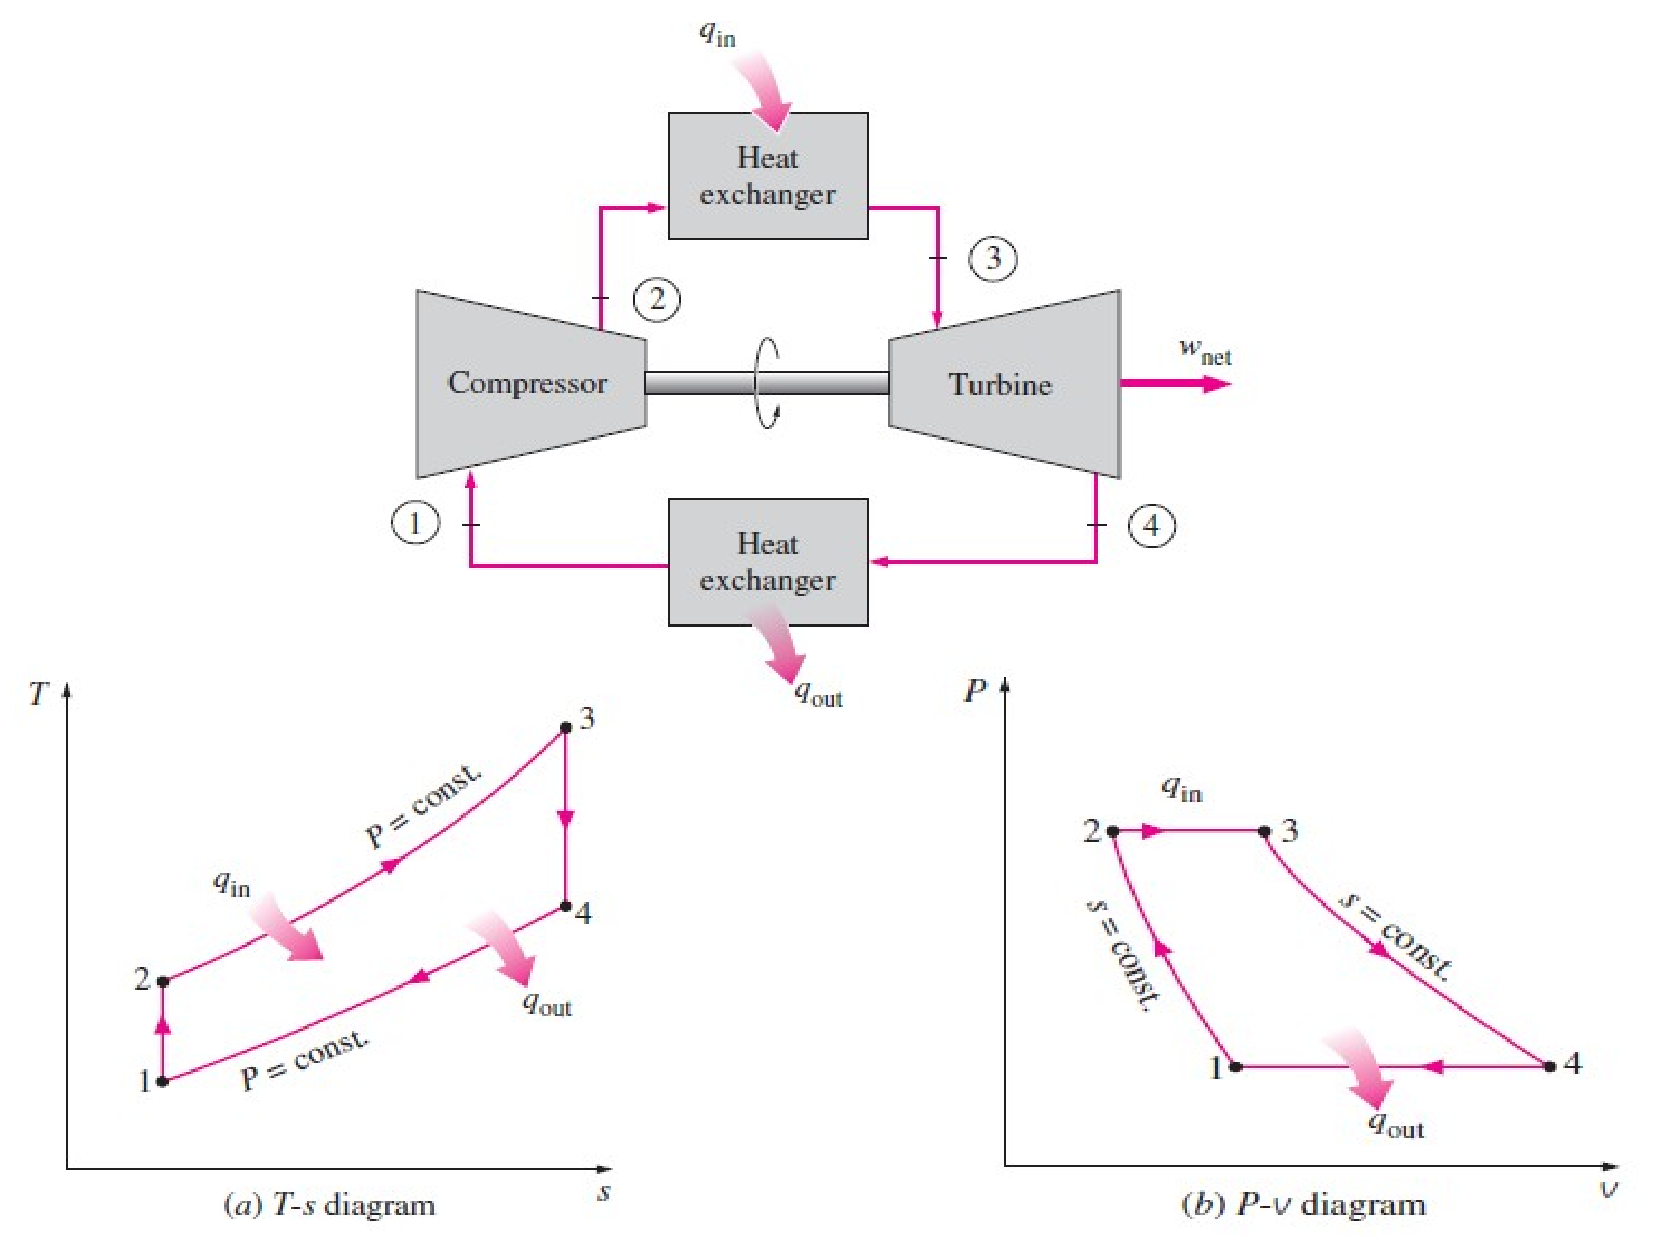
\includegraphics[height=6.cm,width=6.5cm,clip]{./Pics/Brayton_cycle1}
   \end{figure}  
    \end{center}
  \end{column}  
 \end{columns}
\end{frame}



%%%
%%% Slide
%%%
\begin{frame}
 \frametitle{Brayton Cycle -- Internally Reversible Processes}
 \begin{columns}
  \begin{column}[c]{0.4\linewidth} 
   \begin{itemize}
    \item <1-> \textcolor{blue}{3--4} Isentropic expansion (turbine) of air from $\left(T_{3},P_{3},V_{3}\right)$ to $\left(T_{4},P_{4},V_{4}\right)$. No heat flow;
    \item <2-> \textcolor{blue}{4--1} Constant-pressure heat rejection: heat is rejected from the system decreasing the volume -- from $\left(T_{4},P_{4}=P_{1},V_{4}\right)$ to $\left(T_{1},P_{1},V_{1}\right)$. \\
\textcolor{blue}{Heat rejected}: $Q_{out}=mC_{p}\left(T_{4}-T_{1}\right)$
   \end{itemize}
  \end{column}
  \begin{column}[c]{0.6\linewidth}
    \begin{center}
   \begin{figure}%
     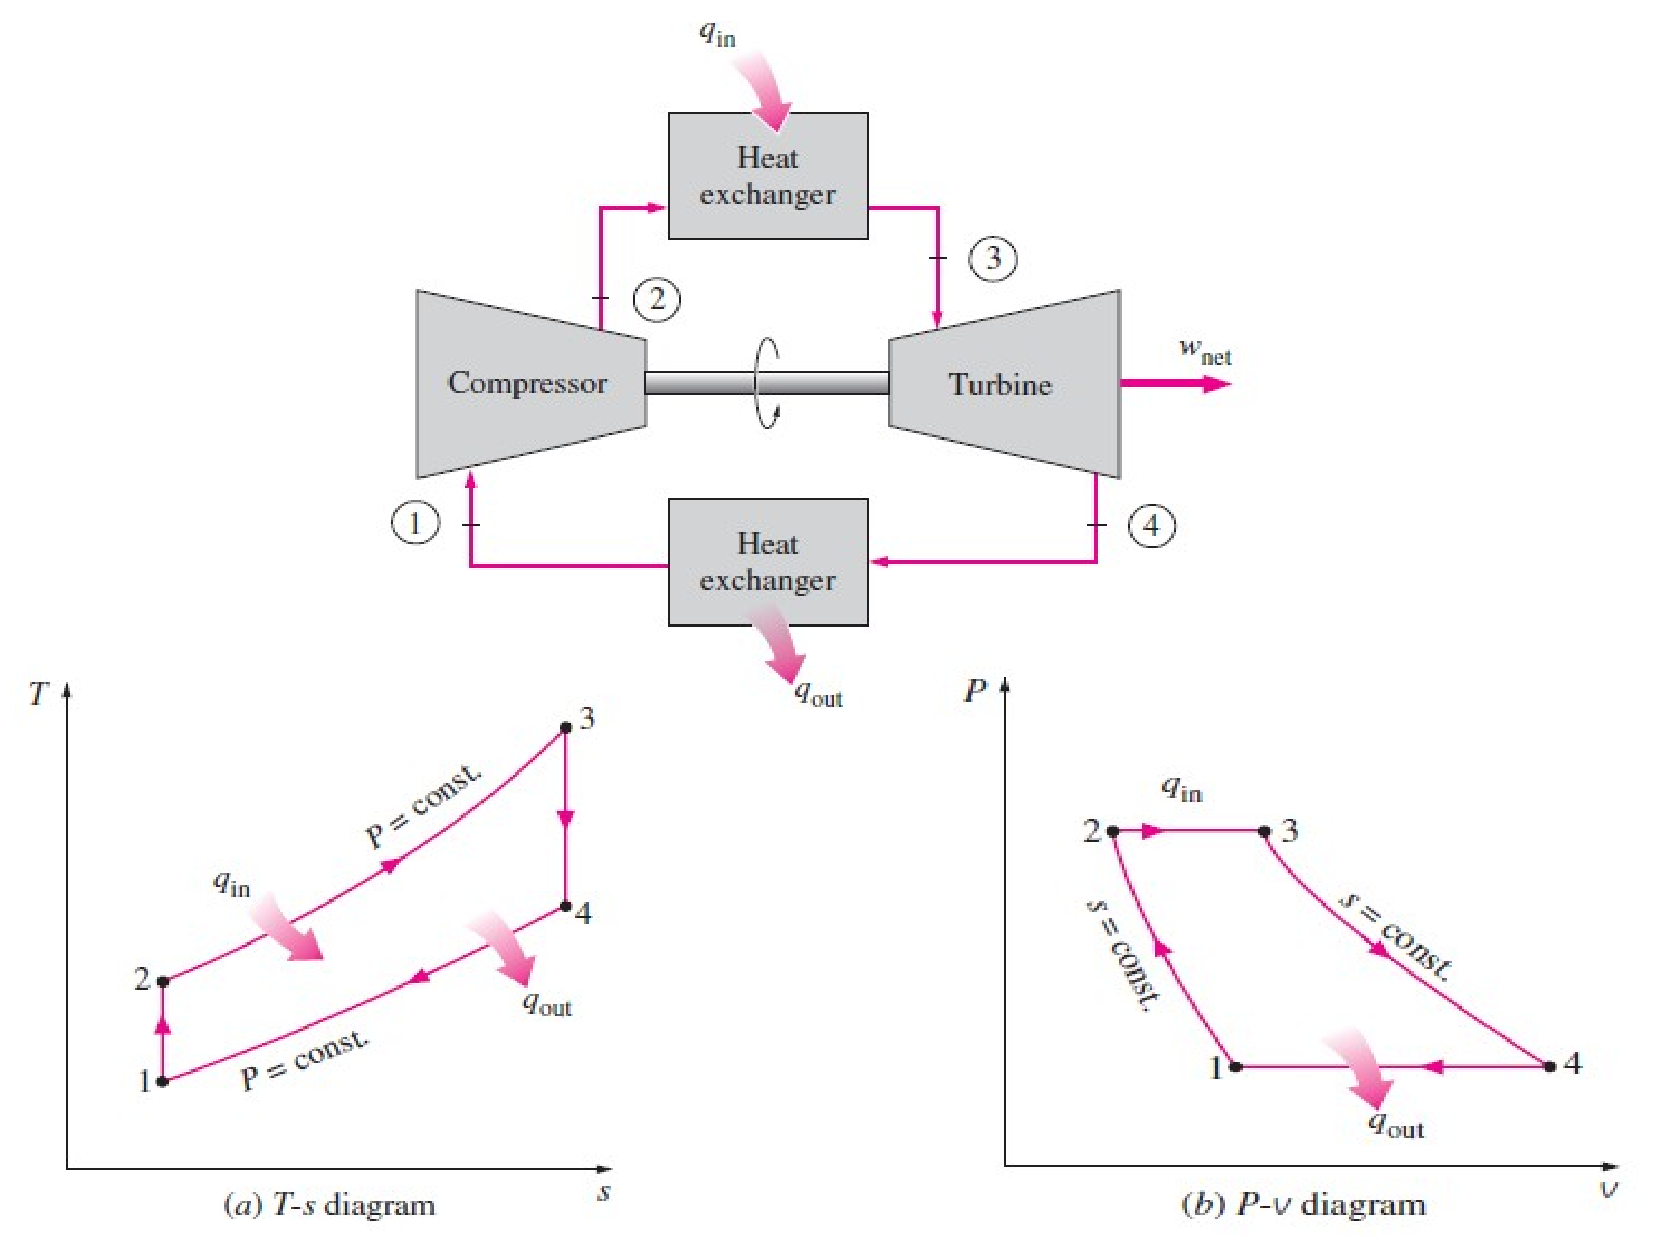
\includegraphics[height=6.cm,width=6.5cm,clip]{./Pics/Brayton_cycle1}
   \end{figure}  
    \end{center}
  \end{column}  
 \end{columns}
\end{frame}




%%%
%%% Slide
%%%
\begin{frame}
 \frametitle{Thermal Analysis}
   Assuming 1 kg of air
   \begin{itemize}
    \item <1-> Net work: 
     \begin{displaymath}
       W_{\text{net}}=C_{p}\left[\left(T_{3}-T_{2}\right)-\left(T_{4}-T_{1}\right)\right]
     \end{displaymath}

    \item <2-> Air-standard Brayton Efficiency 
      \begin{displaymath}
       \textcolor{blue}{\eta_{\text{Brayton}}}= \frc{\text{Net Work}}{\text{Heat Received}}= \textcolor{blue}{1 - \frc{T_{3}-T_{1}}{T_{3}-T_{2}}}
      \end{displaymath}
    
    \item <3-> From the isentropic expansion (3--4) and compression (1--2), we can obtain the $T_{2}$ and $T_{3}$ 
      \begin{displaymath}
         T_{2} = T_{1} r_{p}^{\left(\gamma-1\right)/\gamma} \text{ and } T_{3} = T_{4}r_{p}^{\left(\gamma-1\right)/\gamma}
      \end{displaymath}
     with pressure ratio $r_{p}=P_{2}/P_{1}$
    \item <4-> And substitute $T_{i}$ in the $\eta_{\text{Brayton}}$ expression and obtain the final equation for the air-standard efficiency
     \begin{displaymath}
       \textcolor{blue}{\eta_{\text{Brayton}} = 1 - \frc{1}{r_{p}^{\left(\gamma-1\right)/\gamma}}}
     \end{displaymath}
   \end{itemize}
\end{frame}



%%%
%%% Slide
%%%
\begin{frame}
 \frametitle{Thermal Analysis}
     \begin{displaymath}
       \textcolor{blue}{\eta_{\text{Brayton}} = 1 - \frc{1}{r_{p}^{\left(\gamma-1\right)/\gamma}}}
     \end{displaymath}
 \begin{itemize}
  \item <1-> This expression shows that the \textcolor{blue}{efficiency} of the ideal Brayton cycle \textcolor{blue}{increases with the pressure ratio, $r_{p}$};
  \item <2-> Upper pressure limit is constrained by the limiting temperature of the material of the turbine,
\begin{center}
\textcolor{blue}{Thermodynamics} $\Longleftrightarrow$ \textcolor{green}{Heat Transfer}  $\Longleftrightarrow$ \textcolor{red}{Material Science and Engineering}
\end{center}
 \end{itemize}
\end{frame}


%%%
%%% Slide
%%%
\begin{frame}
 \frametitle{Thermal Analysis}
 \begin{itemize}
  \item <1-> We can easily prove it by using the previously defined net work $\left(W_{\text{net}}\right)$:
    \begin{eqnarray}
       W_{\text{net}}&=&C_{p}\left[\left(T_{3}-T_{2}\right)-\left(T_{4}-T_{1}\right)\right]=C_{p}\left[\left(T_{3}-T_{4}\right)-\left(T_{2}-T_{1}\right)\right] \nonumber \\
                   &=&C_{p}\left[T_{3}\left(1-\frc{T_{4}}{T_{3}}\right)-T_{1}\left(\frc{T_{2}}{T_{1}}-1\right)\right] \nonumber
    \end{eqnarray}
   \item <2-> Since $\frc{T_{3}}{T_{4}}=r_{p}^{\left(\gamma-1\right)/\gamma}=\frc{T_{2}}{T_{1}}$ and assuming $\gamma$ is constant and therefore $\phi=\frc{\gamma-1}{\gamma}$,
    \begin{displaymath}
     W_{\text{net}} = C_{p}\left[T_{3}\left(1-r_{p}^{-\phi}\right)-T_{1}\left(r_{p}^{\phi}-1\right)\right]
    \end{displaymath}
   \item <3-> In order to obtain the maximum net work, we should differentiate $W_{\text{net}}$ with respect to $r_{p}$,
    \begin{displaymath}
     \frc{d}{d r_{p}}W_{\text{net}}= C_{p} \left[ T_{3} \frc{\phi}{r_{p}\left(\phi+1\right)}-T_{1}\phi r_{p}^{\phi-1}\right]=0
    \end{displaymath}
 \end{itemize}
\end{frame}


%%%
%%% Slide
%%%
\begin{frame}
 \frametitle{Thermal Analysis}
 \begin{columns}
  \begin{column}[c]{0.4\linewidth} 
 \begin{itemize}
  \item <1-> Simplifying the previous equation, we obtain, 
    \begin{displaymath}
         \textcolor{blue}{r_{p}=\left(\frc{T_{3}}{T_{1}}\right)^{\frc{\gamma}{2\left(\gamma-1\right)}}}
    \end{displaymath}
   \item <2-> With $T_{1}$ being the minimum temperature of the system (i.e., inlet compressor temperature) and $T_{3}$ the maximum temperature that the turbine is able to withstand;
   \item <3-> For design purposes, we need to compromise between $r_{p}$ $\left(\text{and therefore }\eta_{\text{Brayton}}\right)$ and the net work output;
 \end{itemize}
  \end{column}
  \begin{column}[c]{0.6\linewidth}
   \begin{itemize}
  \item <4-> With less work output per cycle $\Rightarrow$ Larger mass flow rate $\Rightarrow$ Larger system (for the same power output) $\Rightarrow$ More expensive.
   \end{itemize}
    \begin{center}
   \begin{figure}%
     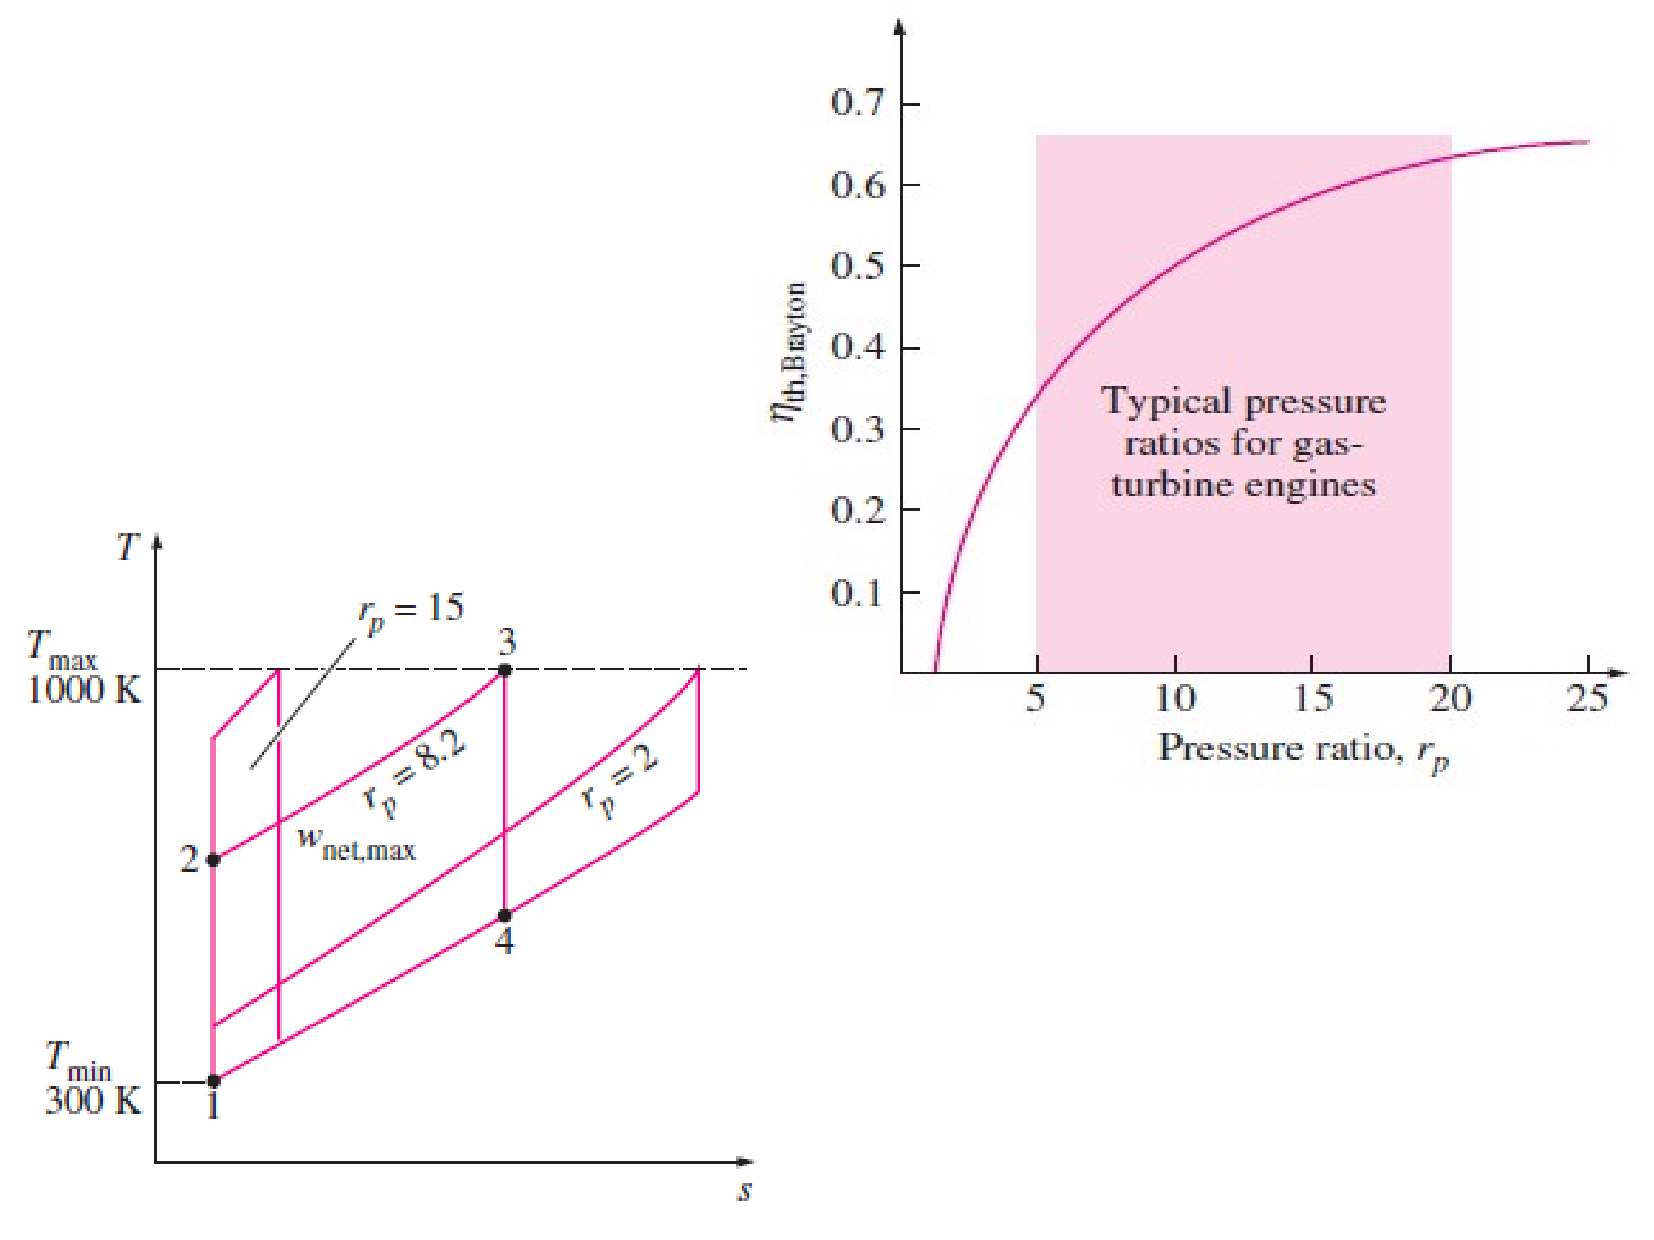
\includegraphics[height=6.cm,width=6.5cm,clip]{./Pics/Brayton_cycle2}
   \end{figure}  
    \end{center}
  \end{column}  
 \end{columns}
\end{frame}


%%%
%%% Slide
%%%
\begin{frame}
 \frametitle{Actual Brayton Cycle -- Open Cycle Gas Turbine}
 \begin{columns}
  \begin{column}[c]{0.4\linewidth} 
 \begin{itemize}
  \item <1-> Real Gas Turbines operate on Open Cycle;
  \item <2-> A rotary compressor and a turbine are mounted on a common shaft;
  \item <3-> Air is driven into a compressor and pumped into a combustion chamber;
  \item <4-> Energy is supplied by spraying fuel into the air stream and;
  \item <5-> The resulting hot gases expand through the turbine to the atmosphere.
 \end{itemize}
  \end{column}
  \begin{column}[c]{0.6\linewidth}
    \begin{center}
   \begin{figure}%
     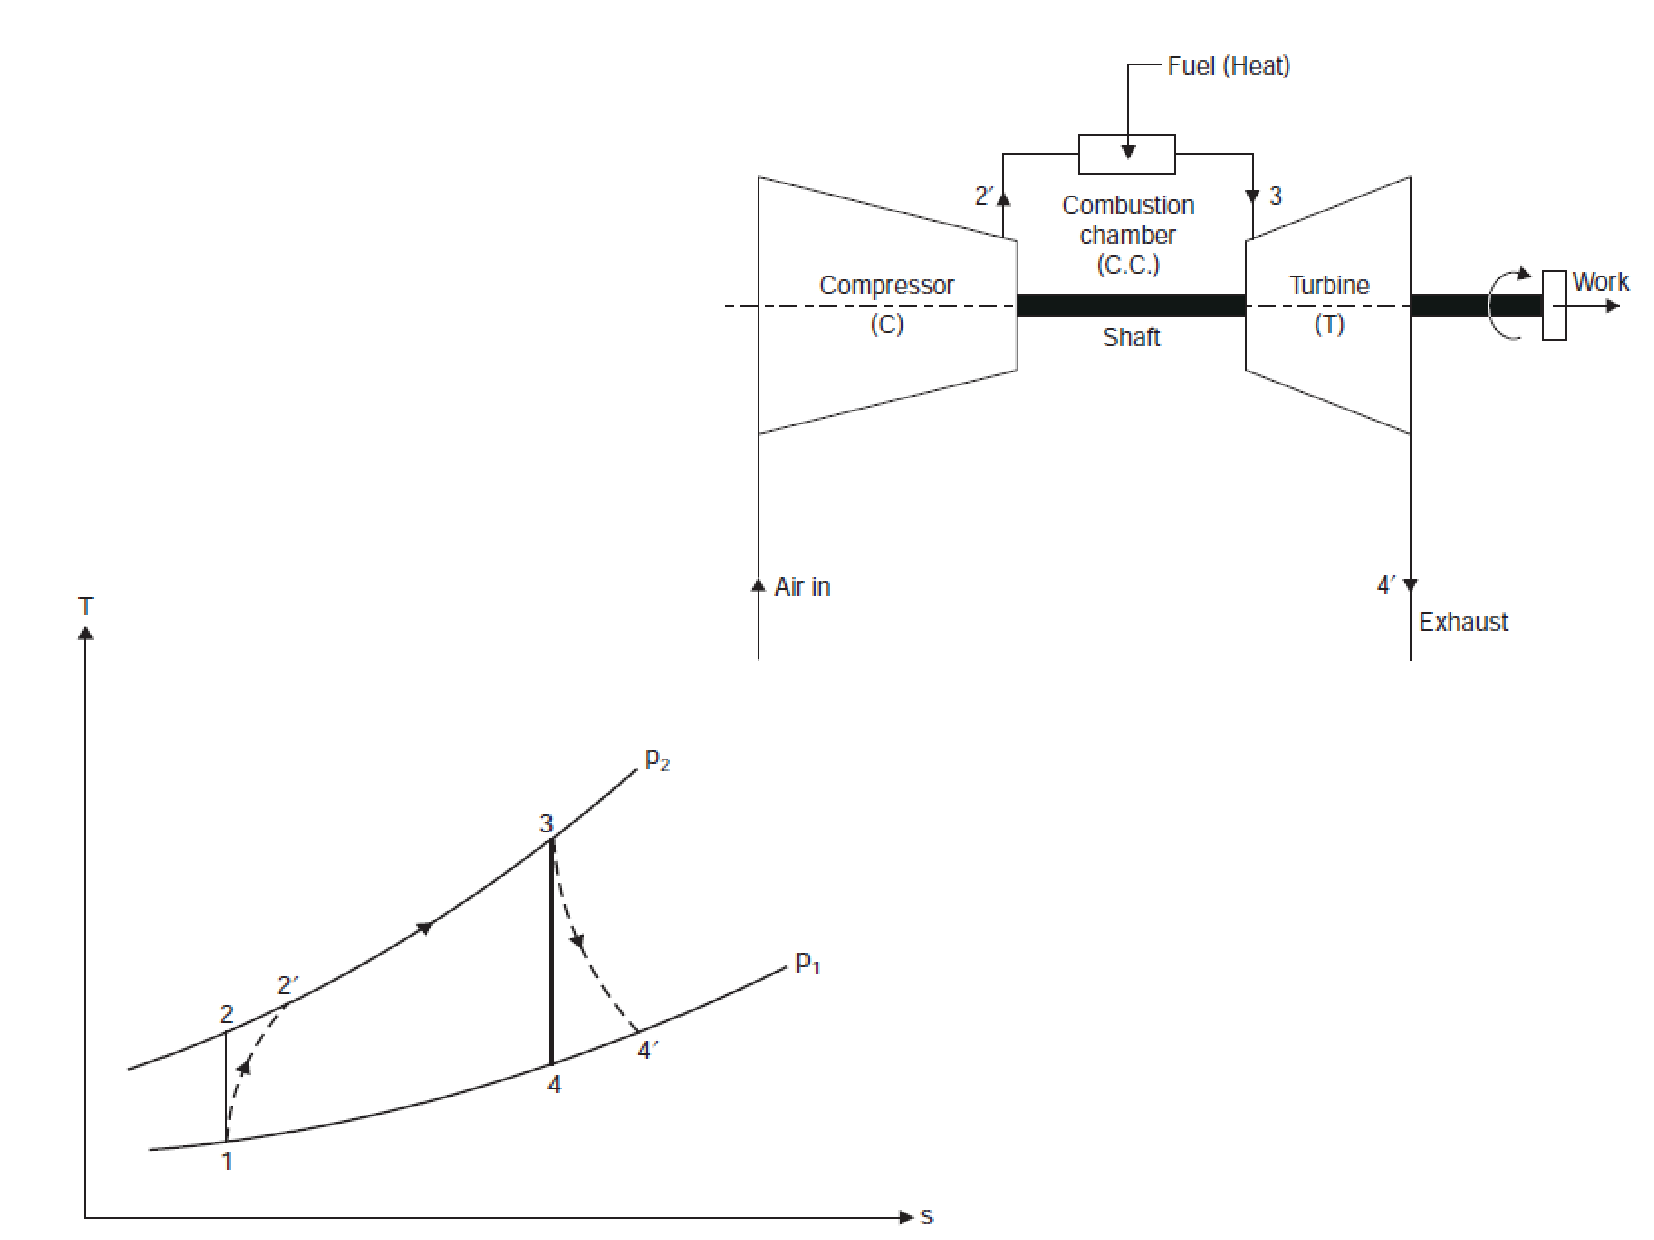
\includegraphics[height=6.cm,width=6.5cm,clip]{./Pics/Brayton_cycle3}
   \end{figure}  
    \end{center}
  \end{column}  
 \end{columns}

\end{frame}


%%%
%%% Slide
%%%
\begin{frame}
 \frametitle{Actual Brayton Cycle -- Open Cycle Gas Turbine}
 \begin{columns}
  \begin{column}[c]{0.4\linewidth} 
 \begin{itemize}
  \item <1-> In order to obtain a net work output from the unit, the turbine must develop more gross work output than is required to drive the compressor and to overcome mechanical losses in the drive;
  \item <2-> The products of combustion coming out from the turbine are exhausted to the atmosphere as they cannot be used any more. The working fluids (air and fuel) must be replaced continuously;
  %\item <3-> If we neglect the pressure loss in the combustion chamber, the actual cycle becomes:
 \end{itemize}
  \end{column}
  \begin{column}[c]{0.6\linewidth}
    \begin{center}
   \begin{figure}%
     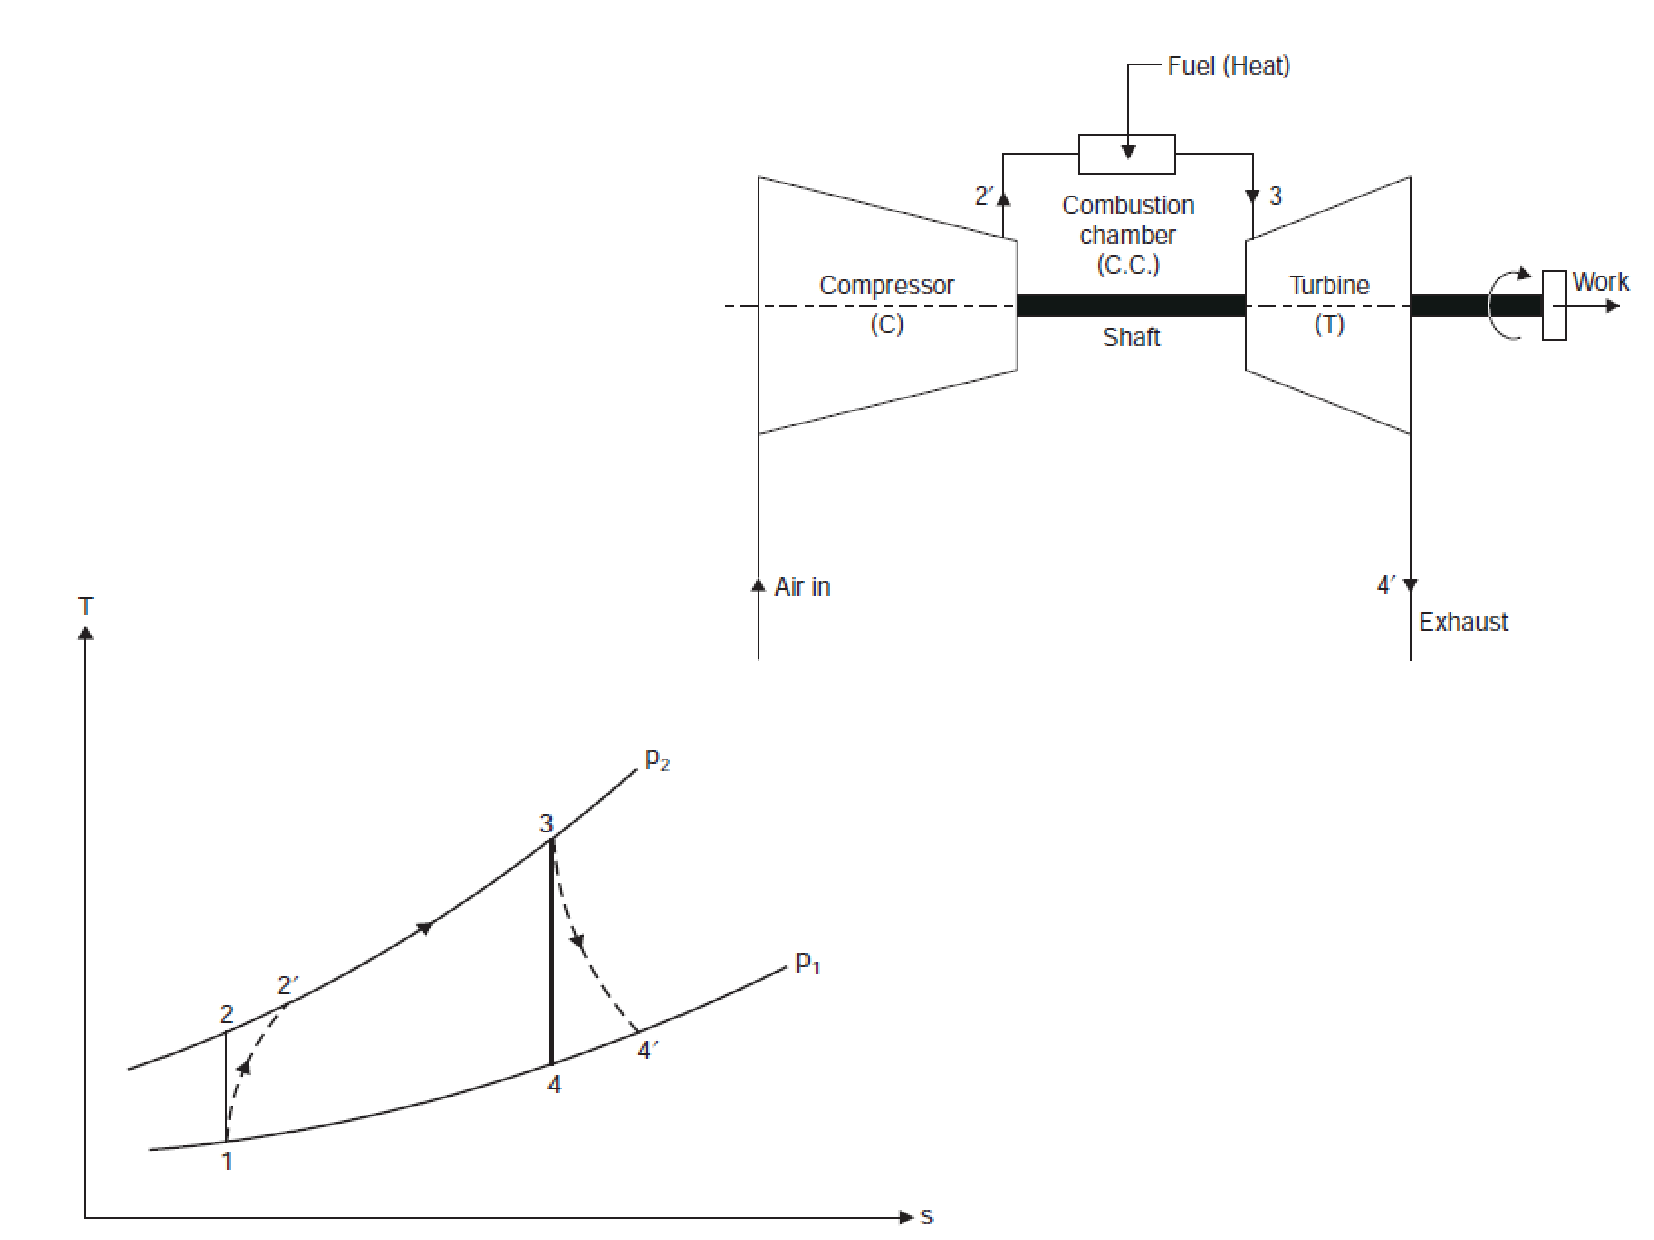
\includegraphics[height=6.cm,width=6.5cm,clip]{./Pics/Brayton_cycle3}
   \end{figure}  
    \end{center}
  \end{column}  
 \end{columns}

\end{frame}


\subsection{Actual Brayton Cycle}
%%%
%%% Slide
%%%
\begin{frame}
 \frametitle{Open Cycle Gas Turbine}
 \begin{columns}
  \begin{column}[c]{0.4\linewidth} 
If we neglect the pressure loss in the combustion chamber, the actual cycle becomes ($Ts$ diagram, rhs):
 \begin{itemize}
  \item <1-> \textcolor{blue}{1--2$^{\prime}$} Irreversible adiabatic compression
  \item <2-> \textcolor{blue}{2$^{\prime}$--3} Constant pressure heat supply in the combustion chamber;
  \item <3-> \textcolor{blue}{3--4$^{\prime}$} Irreversible adiabatic expansion;
  \item <4-> \textcolor{blue}{1--2} Ideal isentropic compression and;
  \item <5-> \textcolor{blue}{3--4} Ideal isentropic expansion.
 \end{itemize}
  \end{column}
  \begin{column}[c]{0.6\linewidth}
    \begin{center}
   \begin{figure}%
     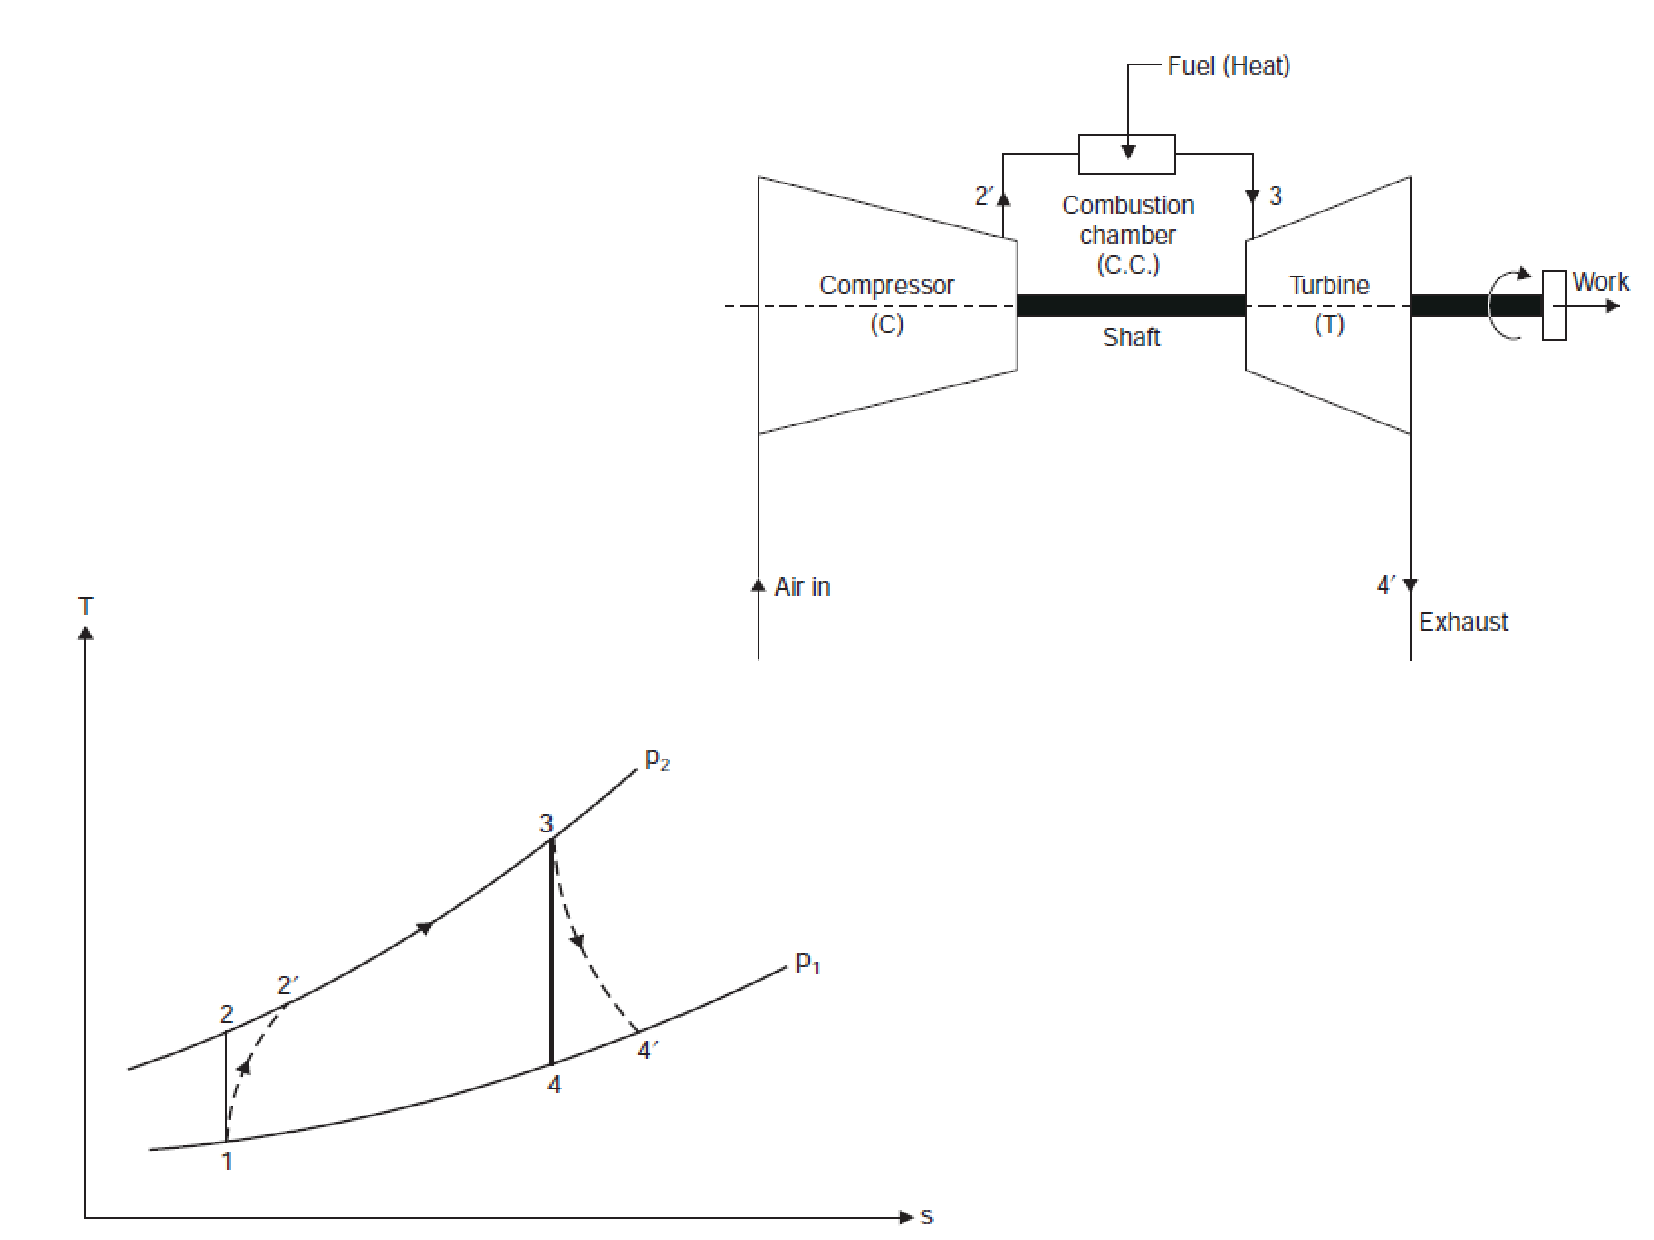
\includegraphics[height=6.cm,width=6.5cm,clip]{./Pics/Brayton_cycle3}
   \end{figure}  
    \end{center}
  \end{column}  
 \end{columns}

\end{frame}



%%%
%%% Slide
%%%
\begin{frame}
 \frametitle{Thermal Analysis}
 \begin{itemize}
  \item <1-> We can still simplify the system by assuming that the change in the kinetic energy in various stages of the cycle is negligible if compared with the enthalpies changes;
  \item <2-> Work input in the compressor: $C_{p}\left(T_{2}^{\prime}-T_{1}\right)$
  \item <3-> Heat supplied in the combustion chamber: $C_{p}\left(T_{3}-T_{2}^{\prime}\right)$
  \item <4-> Work output from the turbine: $C_{p}\left(T_{3}-T_{4}^{\prime}\right)$
  \item <5-> Net work: $W_{\text{net}}=C_{p}\left[\left(T_{3}-T_{4}^{\prime}\right) - \left(T_{2}^{\prime}-T_{1}\right)\right]$
  \item <6-> And the thermal efficiency,
      \begin{displaymath}
       \textcolor{blue}{\eta_{\text{Thermal}} = \frc{\left(T_{3}-T_{4}^{\prime}\right) - \left(T_{2}^{\prime}-T_{1}\right)}{T_{3}-T_{2}^{\prime}}}
      \end{displaymath}
  \item <7-> The efficiency of the isentropic compressor:
      \begin{eqnarray}
        \textcolor{blue}{\eta_{\text{Comp}}}&=&\frc{\text{Work input in the isentropic compressor}}{\text{Actual work required}} \nonumber \\
                                          &=& \textcolor{blue}{\frc{T_{2}-T_{1}}{T_{2}^{\prime}-T_{1}}}\nonumber
      \end{eqnarray}
 \end{itemize}
\end{frame}



%%%
%%% Slide
%%%
\begin{frame}
 \frametitle{Thermal Analysis}
 \begin{itemize}
  \item <1-> And the efficiency of the isentropic turbine:
      \begin{eqnarray}
        \textcolor{blue}{\eta_{\text{Turb}}}&=&\frc{\text{Actual work output}}{\text{Isentropic work output}} \nonumber \\
                                          &=& \textcolor{blue}{\frc{T_{3}-T_{4}^{\prime}}{T_{3}-T_{4}}}\nonumber
      \end{eqnarray}
   \end{itemize}
\end{frame}


%%%
%%% Slide
%%%
\begin{frame}
 \frametitle{Improving the Efficiency}
 \begin{columns}
  \begin{column}[c]{0.5\linewidth} 
 \begin{itemize}
  \item <1-> \textcolor{blue}{Intercooling:} the compressor utilises the larger percentage of power developed by the gas turbine. The work required by the compressor can be reduced by compressing the air in two stages and incorporating an intercooler between the two; 
  \item <2-> \textcolor{blue}{Reheating:} The output of a gas turbine can be improved by expanding the gases in two stages with a reheater between the two. The HP turbine drives the compressor and the LP turbine provides the useful power output. 
 \end{itemize}
  \end{column}
  \begin{column}[c]{0.5\linewidth}
    \begin{center}
   \begin{figure}%
     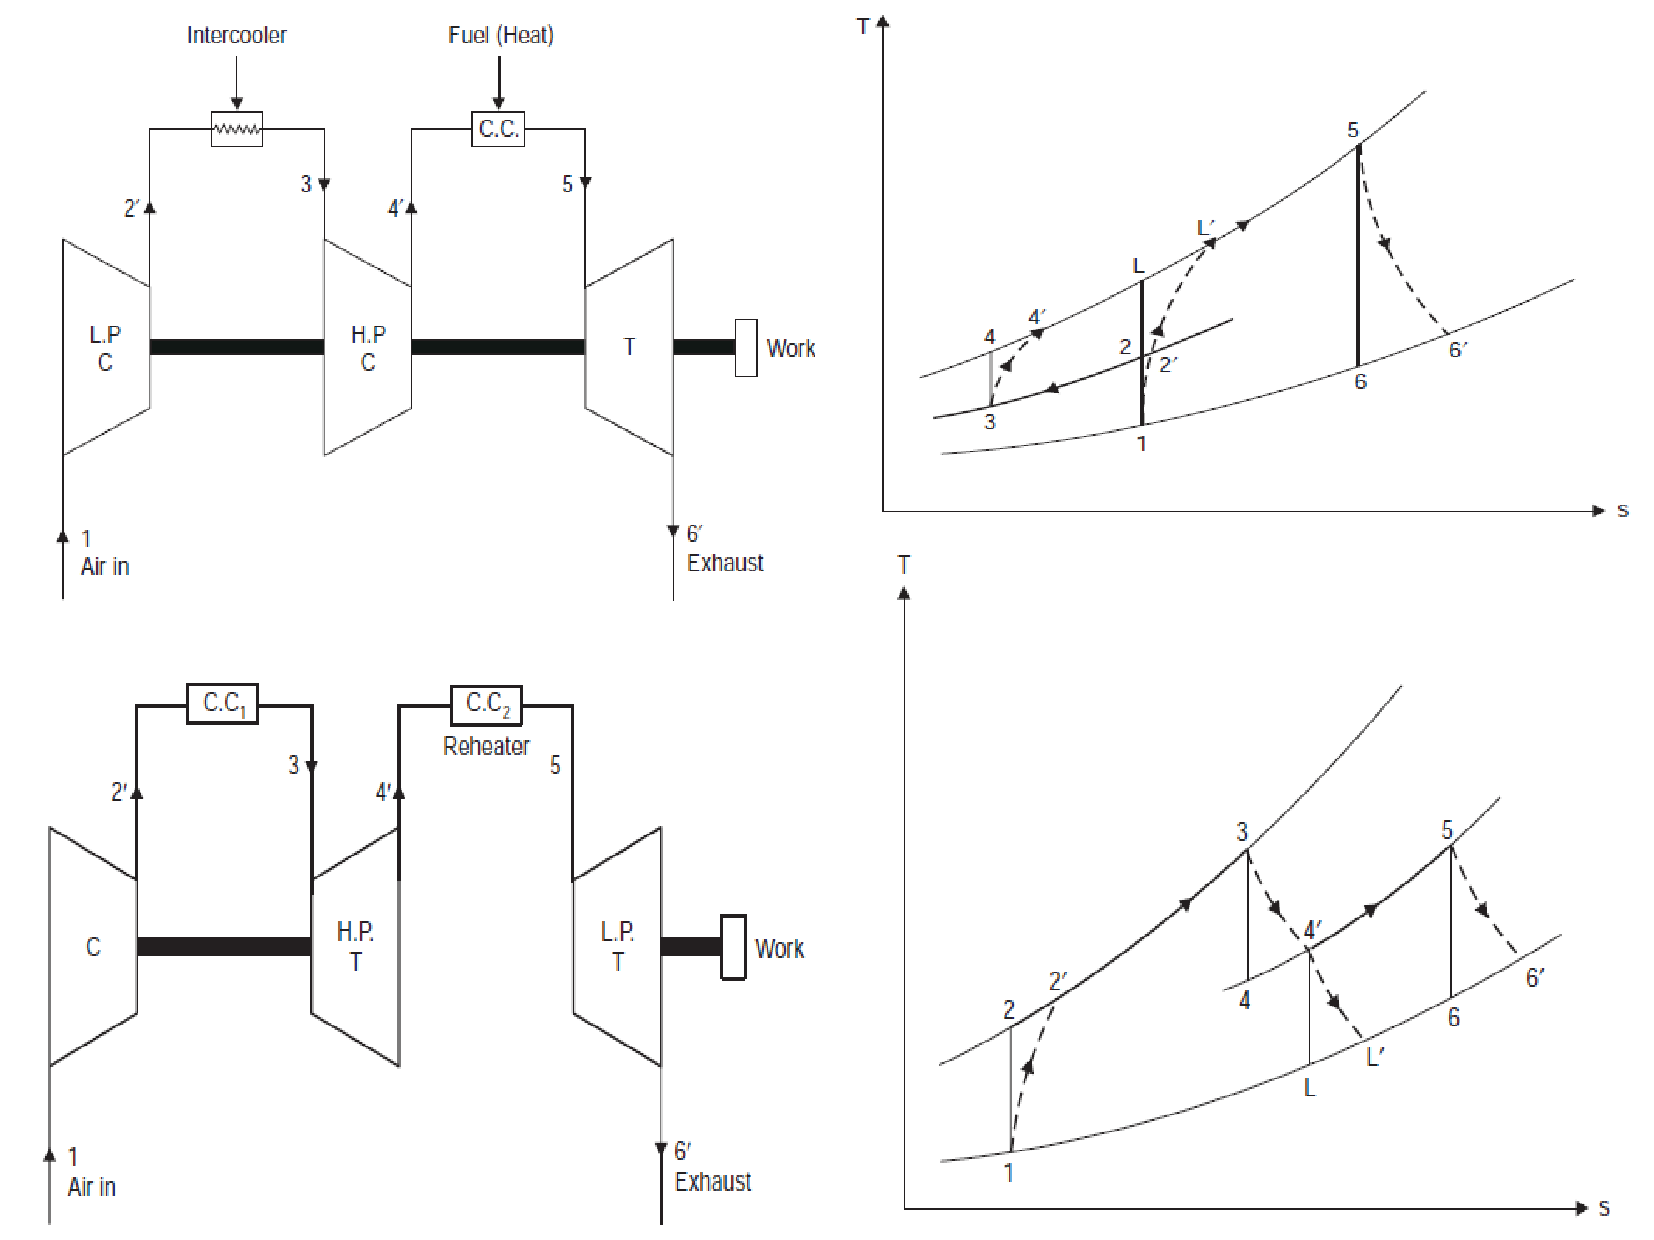
\includegraphics[height=6.cm,width=6.5cm,clip]{./Pics/Brayton_cycle7}
   \end{figure}  
    \end{center}
  \end{column}  
 \end{columns}
\end{frame}


%%%
%%% Slide
%%%
\begin{frame}
 \frametitle{Improving the Efficiency: Brayton Cycle with Regeneration}
 \begin{columns}
  \begin{column}[c]{0.4\linewidth} 
 \begin{itemize}
  \item <1-> Temperature of the exhaust gasses leaving the turbine, $T_{4}$ is higher than the temperature leaving the compressor $T_{2}$ leading the combustion chamber;
  \item <2-> In order to improve the efficiency of the cycle we can use part of the heat from the $T_{4}$ fluid stream to increase the temperature of flow leaving the compressor;
  \item <3-> To this end, we can use a \textcolor{blue}{counter-flow heat exchanger}. This is also known as \textcolor{blue}{regenerator} or \textcolor{blue}{recuperator}.
 \end{itemize}
  \end{column}
  \begin{column}[c]{0.6\linewidth}
    \begin{center}
   \begin{figure}%
     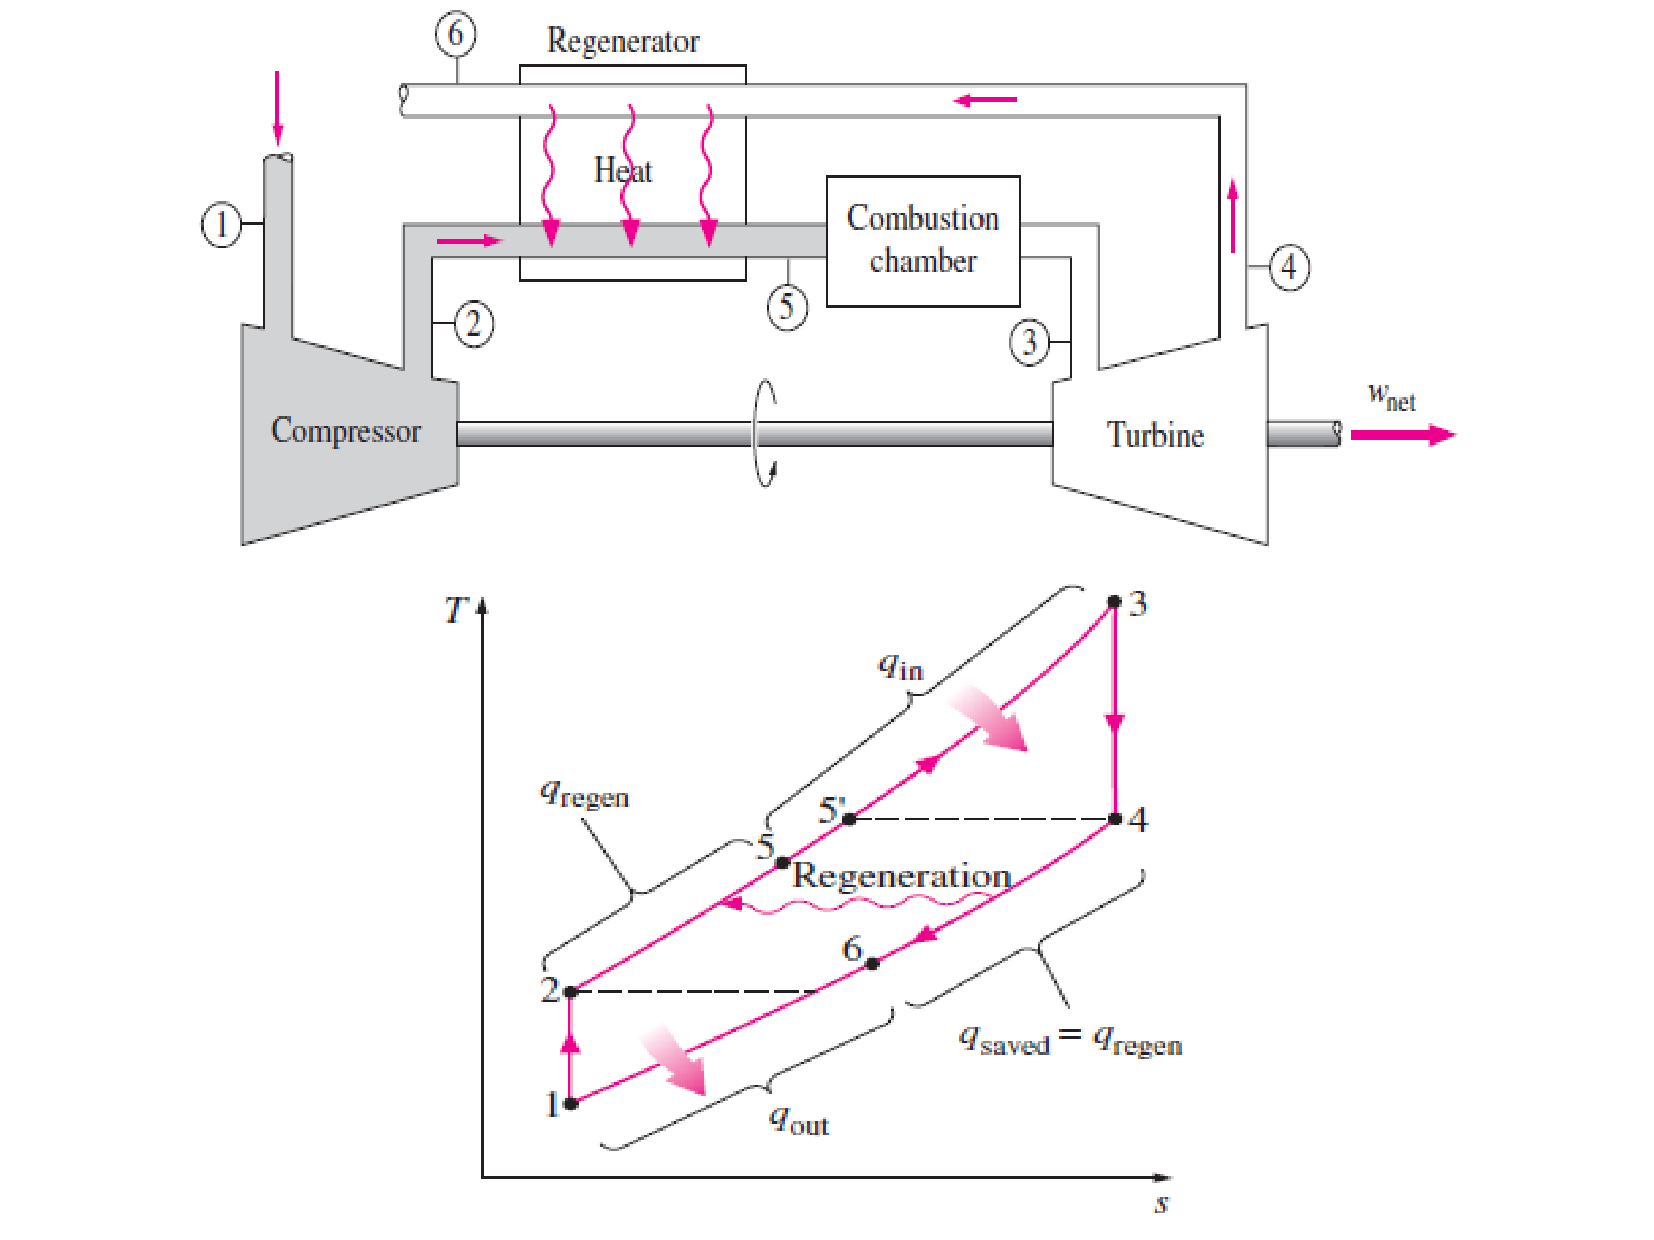
\includegraphics[height=6.cm,width=6.5cm,clip]{./Pics/Brayton_cycle4}
   \end{figure}  
    \end{center}
  \end{column}  
 \end{columns}

\end{frame}


%%%
%%% Slide
%%%
\begin{frame}
 \frametitle{Improving the Efficiency: Brayton Cycle with Regeneration}
 \begin{columns}
  \begin{column}[c]{0.4\linewidth} 
 \begin{itemize}
  \item <1-> Notice that $T_{5^{\prime}}=T_{4}>T_{5}$
  \item <2-> The extent to which a regenerator approaches an ideal regenerator is called \textcolor{blue}{effectiveness}, $\varepsilon$
   \begin{displaymath}
     \textcolor{blue}{\varepsilon=}\frc{Q_{\text{Regen}}^{\text{act}}}{Q_{\text{Regen}}^{\text{max}}} = \textcolor{blue}{\frc{h_{5}-h_{2}}{h_{4}-h_{2}}}
    \end{displaymath}
  \item <3-> If we use the air-standard assumptions, the expression above becomes,
   \begin{displaymath}
     \textcolor{blue}{\varepsilon= \frc{T_{5}-T_{2}}{T_{4}-T_{2}}}
    \end{displaymath}   
 \end{itemize}
  \end{column}
  \begin{column}[c]{0.6\linewidth}
    \begin{center}
   \begin{figure}%
     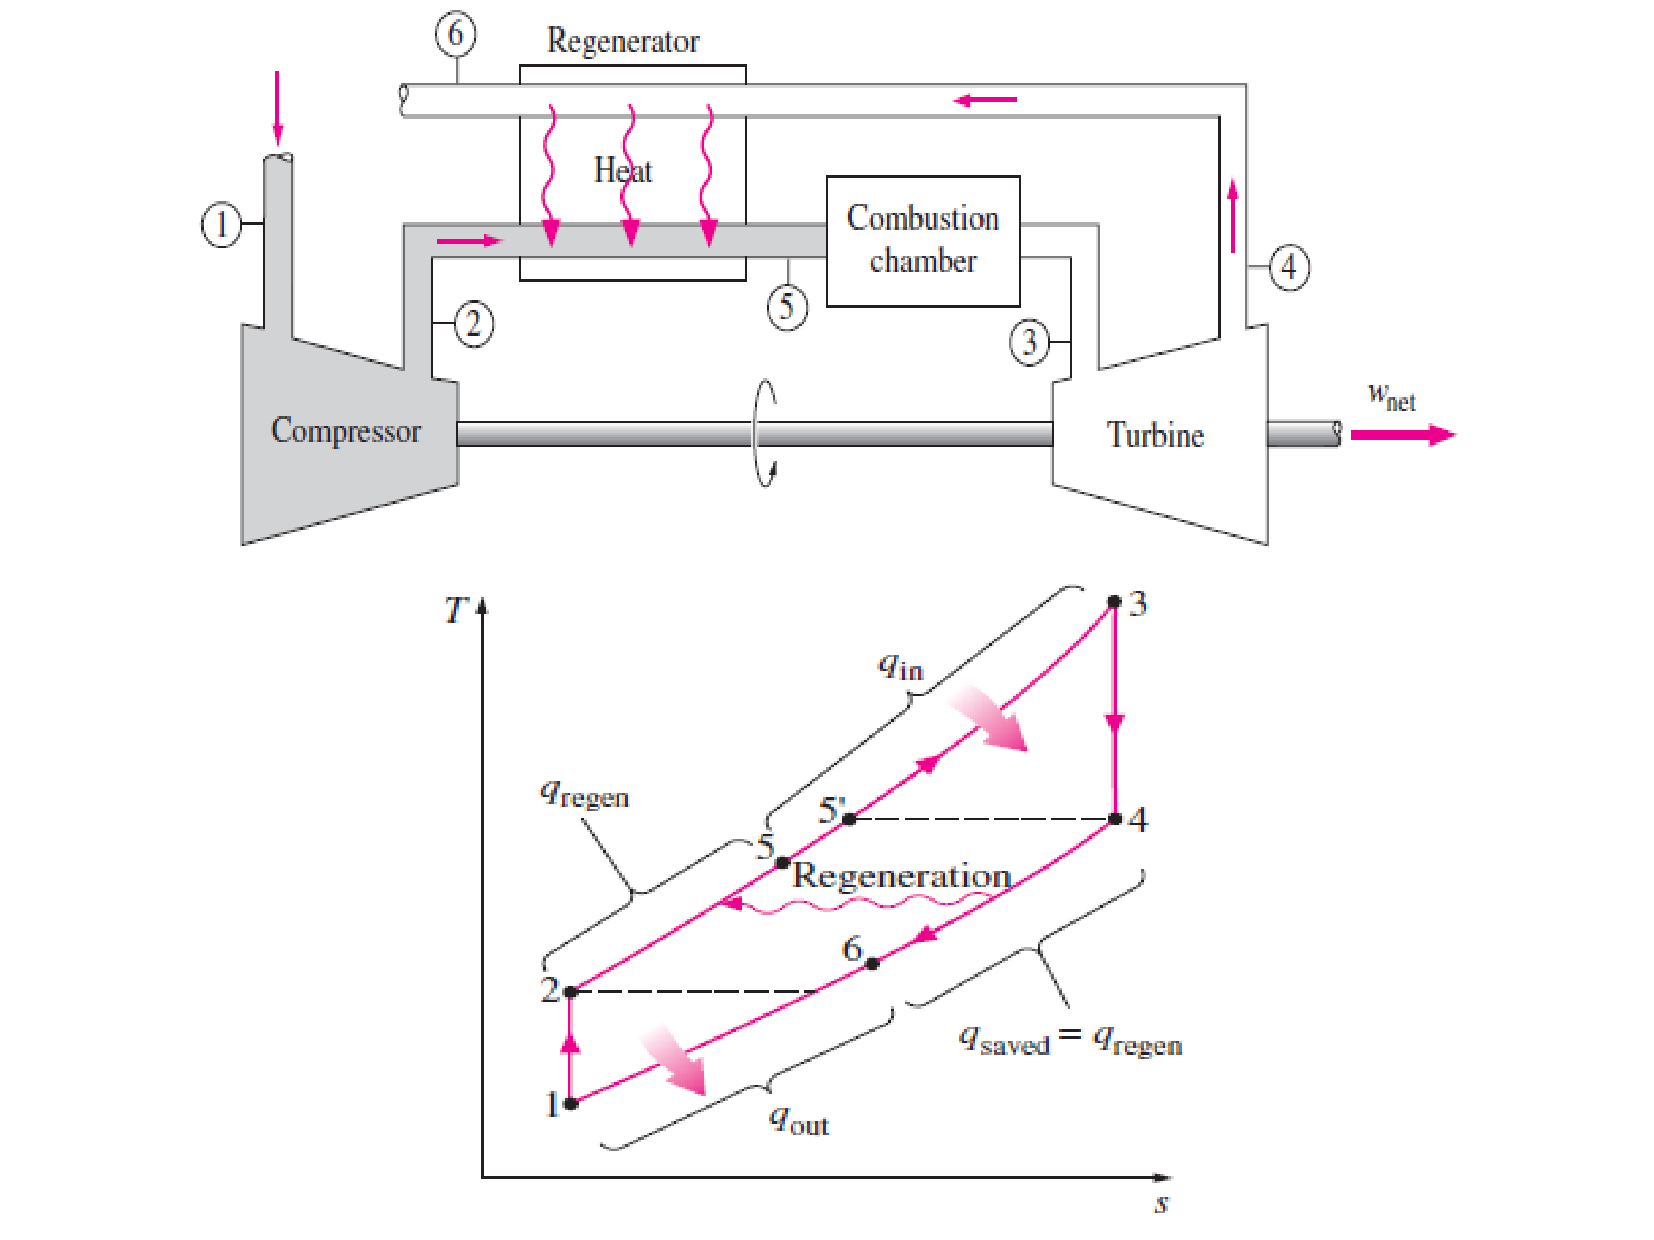
\includegraphics[height=6.cm,width=6.5cm,clip]{./Pics/Brayton_cycle4}
   \end{figure}  
    \end{center}
  \end{column}  
 \end{columns}

\end{frame}


%%%
%%% Slide
%%%
\begin{frame}
 \frametitle{Improving the Efficiency: Brayton Cycle with Regeneration}
 \begin{columns}
  \begin{column}[c]{0.4\linewidth} 
 \begin{itemize}
  \item <1-> A regenerator with a higher effectiveness obviously saves a greater amount of fuel since it preheats the air to a higher temperature prior to combustion;
  \item <2-> The effectiveness of most regenerators used in practice is below 0.85;
  \item <3-> The thermal efficiency of the Brayton cycle with regenerator is
    \begin{displaymath}
     \textcolor{blue}{\eta_{\text{Brayton}}^{\text{Regen}}= 1 - \left[\frc{T_{1}}{T_{3}}\right] r_{p}^{\left(\gamma-1\right)/\gamma}}
    \end{displaymath} 
   
 \end{itemize}
  \end{column}
  \begin{column}[c]{0.6\linewidth}
    \begin{center}
   \begin{figure}%
     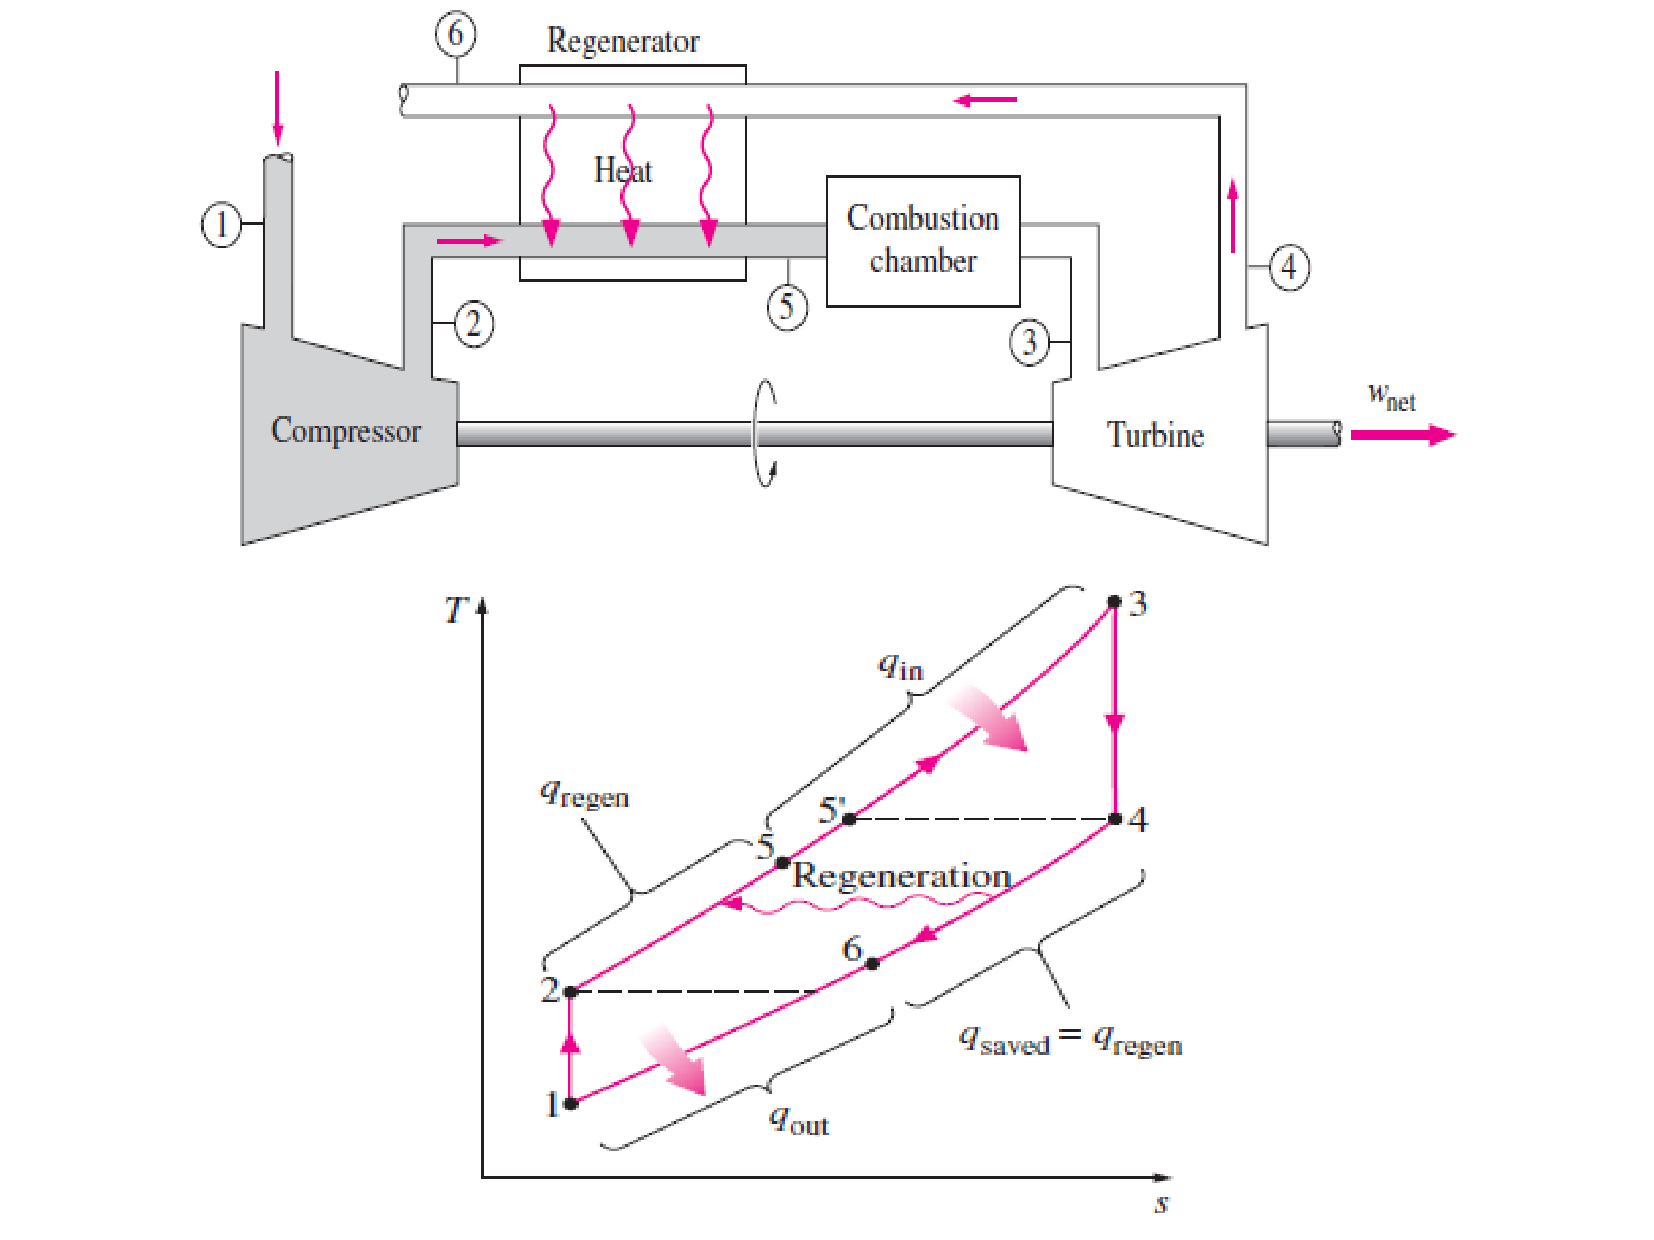
\includegraphics[height=6.cm,width=6.5cm,clip]{./Pics/Brayton_cycle4}
   \end{figure}  
    \end{center}
  \end{column}  
 \end{columns}

\end{frame}


\subsection{Summary}
%%%
%%% Slide
%%%
\begin{frame}
 \frametitle{Summary}
  In this first Module we studied:
  \begin{itemize}
   \item <1-> Review of the fundamentals of thermodynamics:
    \begin{enumerate}
     \item <2-> 0$^{\text{th}}$-3$^{\text{th}}$ Laws;
     \item <3-> Intensive/Extensive properties and derivation of the Second Law;
    \end{enumerate}

   \item <4-> Vapour-based Power Cycles:
    \begin{enumerate}
     \item <5-> Ideal Carnot cycle / engines;
     \item <6-> Rankine and Modified Rankine cycles/ engines;
     \item <7-> Components of the cycles (turbine, compressors, heat exchangers etc);
     \item <8-> Thermal analysis of the cycles / engines based on First and Second Laws;
    \end{enumerate}

   \item <9-> Gas-based Power Cycles:
    \begin{enumerate}
     \item <10-> Internal Combustion:
      \begin{enumerate}
       \item <12-> Reciprocating engines;
       \item <13-> Ideal Carnot cycles;
       \item <14-> Otto, Diesel, Dual Combustion and Atkinson cycles;
       \item <15-> Thermal and sensitivity analysis of the cycles / engines based on First and Second Laws;
      \end{enumerate}
     \item <11-> External Combustion:
        \begin{enumerate}
         \item <16-> Stirling and Ericsson cycles;
         \item <17-> Brayton Gas Turbine Cycles;
         \item <18-> Thermal and sensitivity analysis of the cycles / engines based on First and Second Laws.
        \end{enumerate}
    \end{enumerate}      

  \end{itemize}

\end{frame}

%%%
%%% Slide
%%%
\begin{frame}
 \frametitle{Efficiency for all Gas-based Power Systems:}

%\begin{table}
\begin{tabular}{| l  c |}
\hline
         & Efficiency   \\
\hline
Carnot   &                         \\
Stirling & $1 - \frc{T_{C}}{T_{H}}$ \\
Ericsson &                         \\
\hline
Otto     & $1 - \frc{1}{r^{\gamma-1}}$ \\
\hline
Diesel   & $1 - \frc{1}{r^{\gamma-1}} \left[\frc{\rho^{\gamma}-1}{\gamma\left(\rho-1\right)}\right]$ \\
\hline
Dual     & $1 - \frc{1}{r^{\gamma-1}} \frc{\beta\rho^{\gamma}-1}{\left[\left(\beta-1\right)+\beta\gamma\left(\rho-1\right)\right]}$ \\
\hline
Atkinson & $1- \gamma\left[\frc{r-\alpha}{r^{\gamma}-\alpha^{\gamma}}\right]$ \\
\hline
Brayton  & $1 - \frc{1}{r_{p}^{\left(\gamma-1\right)/\gamma}}$\\
\hline
Brayton with &  \\
Regenerator & $1 - \left[\frc{T_{1}}{T_{3}}\right] r_{p}^{\left(\gamma-1\right)/\gamma}$ \\

\hline

\end{tabular}
%\end{table}

\end{frame}





\end{document}
